\chapter{Beauty and understanding}
\label{chap:beauty}

% 80k chars

This chapter focuses on what beauty has to do with understanding, first from a theoretical perspective, and then diving specifically into how specific domains approach this relation. Our theoretical approach will be based on the aesthetic theory of Nelson Goodman, and a lineage which links aesthetics to cognition, most recently aided by the contribution of neurosciences.

After argumenting for a conception of aesthetics which tends to intellectual, rather than emotional, engagement, we will pay attention to how surface structure and conceptual assemblages relate. That is, we will highlight how each of the domains contigent to source code— literature, mathematics and architecture—communicate certain concepts through their respective and specific means of symbolic representation.

\section{Aesthetics and cognition}
\label{sec:aesthetic-cognition}

%20k characters, doing an overview of how aesthetic philosophy relates to cognition

The way that things are presented formally—which we've defined as their aesthetics—have been empirically shown to affect the comprehension of content. Without engaging too directly in the media-determination thesis, which states that what one can say is determined by the medium through which they say it, be it language or technical media, we nonetheless start from the point that form influences content \citep{postman_amusing_1985}.

Jack Goody and Walter Ong have shown in their anthropological studies that the primary means of communication of the surveyed communities does affect the engagement of said communities with concepts such as ownership, history and governance \citep{ong_orality_2012,goody_logic_1986}. More recently, Edward Tufte and his work on data visualization have furthered this line of research by focusing on the translation of similar data from textual medium to graphic medium \citep{tufte_visual_2001}. A case has indeed been made for the impact of appearance towards structure, both in source code and elsewhere. To complement this comparative approach between several mediums, we now look at how source code performs expressively as a specific system, starting from Nelson Goodman's theorization of such a system..

\subsection{Source code as a language of art}
\label{subsec:source-code-language-art}

From the question of the nature of the aesthetic experience from the perspective of the audience, whether as an aesthetic emotion being felt or as an aesthetic judgment being given, we shift our attention to the object of aesthetic experience, and to the questions of \emph{how does a work represent?} and \emph{what does a work represent?}. To answer these, we rely on answers provided by by Nelson Goodman in the \emph{Languages of Art: An Approach to a Theory of Symbols} \citep{goodman_languages_1976} and \emph{The Structure of Appearance} \citep{goodman_structure_1966}.

The starting point for Goodman's analysis is that production and understanding in the arts involve human activities that, though they differ in specific ways among themselves and from other activities, are nevertheless generically related to perception, scientific inquiry, and other cognitive activity, and such an activity specifically involves symbolic systems. It is those two components that Goodman aims at expliciting: what constitutes an aesthetic symbol system, and how does it express?

Goodman develops a systematic approach to symbols in art, freed from any media-specificity (e.g. from pictorial symbols to musical notations and even time marks on clocks and watches). A symbolic system, in his definition, consists of characters, along with rules to govern their combination with other characters, itself correlated with a field of reference. These symbols and their arrangement within a work of art supports an aesthetic experience\footnote{It should be noted here that Goodman does not limit the aesthetic experience to a positive, pleasurable one. An artistic symbolic system can be seen even if the result is considered bad.}. A work, as a part, particular arrangement of a symbol system according to specific syntactic and semantic rules, can therefore enable an aesthetic experience.

A symbol system is based on five requirements: a system should be composed of signs which are unambiguous, syntactically and semantically disjointed, and differentiated \citep{goodman_languages_1976}. This classification makes it possible to compare the various symbolization systems used in art, science, and life in general: from clocks to counters, from diagrams to maps models, from musical scores to painters' sketches and scripts (intended in a broad sense as the characters of natural languages). In our case, this provides us for a framework to investigate the extent to which source code qualifies as a language of art.

Source code is written in a formal linguistic system called a programming language. Such a linguistic system is, obviously, digital in nature, and therefore satisfies at least the syntactic requirements of disjointedness, differentiation (a mark only ever corresponds to that symbol, such as a variable or function name), as well as syntactic repleteness (relatively fewer factors need to be taken into account during the interpretative process)\footnote{This does not mean that any program text written in this symbolic system will tend to be syntactically replete. On the contrary, the tendency of program text to veer towards verbosity implies the desirable state of repleteness.}. This does qualify source code as a potential language for art, through which aesthetic expressiveness can emerge.

As Goodman notes, the distinct signs that compose a symbols system do not have intrinsic properties, but a thing serves as a sign only in relation to a symbol system, and a field of reference. Some requirements need to be fulfilled for such a symbol to be what is called a symptom of the aesthetic. Amongst exemplification, syntactic density, semantic density and syntactic repleteness, source code fulfills the last two criteria: with a limited set of symbols (at one of the lowest levels, only two symbols, traditionally marked as 0 and 1), programs can refer to and enact complex states and behaviours.

The field of reference is understood her as being the set of concepts which are being referred to by a symbolic system. For instance, a symbolic system such as western classical music can refer to concepts such as lament, piety, heroism or grace, while a chine \emph{shanshui} painting has a landscape composed of mountains and rivers as its field of reference. The combination of both the problem domain, as evoked in \ref{chap:understanding}, and of the technological environment on which the source code is to be executed, is posited here as an equivalent to the Goodman's field of reference.

Now that we have highlighted what a symbolic system is, we turn to how such a system can signify and reference a particular field of reference.

Goodman highlights the ways in which symbols systems communicate, through the notion of \emph{reference}. To refer to, in this sense, is the action by which a symbol stands in for an item. Reference, he sketches out, takes place through the different dyads of denotation and exemplification, description and representation, possession and expression \citep{goodman_languages_1976}. We will see how these various means of referring can be instantiated in the symbolic system of source code.

First, then, denotation; it is the core of representation, a reference from a symbol to one or many objects it applies to and is independent of resemblance. Rather, it uses a particular relationship via the use of labels; that is, a symbol stands in for an item in the field of reference. For instance, a name denotes its bearer and a predicate each object in its extension. Names such as variable names or function names thus denote a particular item in the field of reference, and act as their label. For instance, \lstinline{var auth_level} denotes an ability to access and modify resources.

The labelling process therefore serves as the symbolic expression for a particular field. In source, this can happen through variable naming (as seen above), but also through type definition\footnote{For instance, a particular choice of a numeric value, such as \lstinline{int} or \lstinline{float} denote a particular level of preciseness}, as well as additional affordances which we look at in \ref{sec:programming-aesthetic-framework}.

Source code also make extensive use of description. If we consider a program text as a series of steps, a series of states, or a series of instructions, then it follows that source code is leaning heavily on the side of description, when it comes to its power of reference. Indeed, a program text is a description of how to solve a problem from the computer's perspective, written extensively in machine language\footnote{Pseudo-code is therefore a representation of a potential source code written in a specific language.}. All source code can therefore be said to be a description of a combination of action and states.

States are also a particular case in source code: they are both a description and, because they are not the thing itself, they are also a representation. As one can see in \ref{code:representation}, an individual can be represented within source code with a particular construct (here called a \lstinline{struct}).

\begin{listing}
    \inputminted{rust}{./corpus/representation.rs}
    \caption{An example of how source code can be a representation an individual, and can exemplify encapsulation, written in Rust.}
    \label{code:representation}
\end{listing}

This representation, in the specific instance of object-oriented programming in \ref{code:representation}, also manifests Goodman's aesthetic symptom of possession. Here, the source code posseses similar properties as the thing referenced (since our prototypal image of a person has an age, a name and interests). Through this possession of a property, it acts as an example of a prototypal person.

Exemplification is another aspect of Goodman's theory, which has nonetheless remained somewhat limited \citep{elgin_making_2011}. A symbol exemplifying, also called an examplar, is considered as a stand-in for an item in the field of reference. Specifically for source, code, this is a case that we have seen in \ref{subsec:scientists}, where a particular source code is written in order to act as an example of a broader concept. For instance, a program text can, at a lower level, exemplify a particular kind of procedure, such as encapsulation or nestedness. The program text therefore exemplifies the constitutive element of the linked list\footnote{A linked list is a basic data structure in computer science, which consists in a succession of connected objects.}. However, a similar program text can also be an example of cleanliness, of clarity, or elegance (see \ref{sec:ideals-beauty}): a program text written by a software developer can be seen as possessing the property of cleanliness, by virtue of its implementation of syntactic and semantic rules, while another program text written by a hacker can be seen as highlighting detailed hardware knowledge.

Additionally, the features a symbol exemplifies depends on its function (or, more precisely, its functional context) \citep{elgin_understanding_1993}. A symbol can perform a variety of function: a piece of code in a textbook might exemplify an algorithm, while the same piece of code in production software might be seen as a liability, or as a boring section in a code poem.

Source code maintains specific features on its relation to the field of reference. On the one hand, a particular class of characters employed as symbols (also called \emph{tokens} in the context of programming languages), do not maintain a clear relationship with the items in the field of reference. That is, in program texts, two distinct symbols can be referring to the same concept, value, or place in memory (see \ref{chap:programming} for a further explanation of these differences and \ref{code:multiple_references} for an example), something Goodman nonetheless assigns as another symptom of the aesthetic: multiple and complex references.

\begin{listing}
    \inputminted{rust}{./corpus/multiple_references.rs}
    \caption{The system of value, references and pointers make source code into a highly complex symbolic system.}
    \label{code:multiple_references}
\end{listing}

% case in point: https://github.com/torvalds/linux/blob/d158fc7f36a25e19791d25a55da5623399a2644f/fs/ext4/resize.c#L698

On the other hand, the representation of a field of reference is done through a disjointed and differentiated system: the boundaries of each items in the field of reference are clearly defined, in virtue of the specific symbol system that programming languages are. These programming languages do dictate the rules of engagement of the symbolic system with the field of reference.

We have shown here that source code qualifies as a symbolic system susceptible of affording symptoms of the aesthetic. We have also highlighted its specificities, particularly in terms of descriptions and representations, and of complex and multiple references. Source code being a dual language, between human and machine, makes it have such complex and multiple references. A final aspect to investigate is the expressiveness of source code, with a particular attention to how source code can manifest of metaphorical exemplification and representation.

The particular expressive power of an aesthetic experience surfaces when the examplification involves a foreign element, an event that Goodman refers to as metaphorical exemplification. While this approach has been broadened by Lakoff et. al., and mentioned in \ref{subsec:metaphor-computation}, philosophers of art have pinpointed the metaphorical event as a reliable symptom of the aesthetic.

Max Black initiates a view of metaphors which go beyond a simple comparison; dubbed the \emph{interaction view}, he considers the metaphorical device as containing positive cognitive content. Simply paraphrasing a metaphor, even if one captures precisely the same connotations/associations as the metaphor, does not convey the same meaning as the metaphor itself\footnote{For instance, saying \emph{Je chavire dans l'écume des phénomènes} does not have the similar expressive power as listing all the properties of \emph{phénomènes}. The original sentence is from Beckett.}.

Through his contribution to aesthetic philosophy, Monroe Beardsley's started touching upon metaphor from a semantic perspective. Published alongside his inquiries into the aesthetic character of an experience, and taken later on by Ricoeur as a basis for his study, \emph{The Metaphorical Twist} implies that semantics and aesthetics might be connected through the structuring operation of the metaphor—that which elicits an aesthetic experience can do so through the creation of unexpected, or previously unattainable meaning. Ricoeur's theory of the metaphor indeed builds on Beardsley's conception that metaphor can have a designative role (the primary subject) which adds a \emph{"local texture of irrelevance"}, a \emph{"foreign component"}, whose semantic richness might over-reach and obfuscate the intended meaning, as well as a connotative one (the secondary subject), in which meaning is peripheral. The cognitive stimulation and enlightment takes place through a metaphor-induced tension, between central and periphery, between illuminating and obfuscating, between evidence and irrelevance.

As Beardsley inquiries into the features necessary for an aesthetic experience, of which the metaphor is part, he lists five criteria to distinguish the character of such an experience. Besides object-directedness, felt-freedom, detached-affect and wholeness, is the criteria of \emph{active discovery}, which is

\begin{quote}
    "a sense of actively exercising the constructive powers of the mind, of being challenged by a variety of potentially conflicting stimuli to try and make them cohere; exhilaration in seeing connections between percepts and meanings; a sense of intelligibility"\footnote{The Aesthetic Experience, in The Aesthetic Point of View \citep{beardsley_aesthetic_1970}.}
\end{quote}

As such, Beardsley highlights the possibility of an aesthetic experience to make understandable, to unlock new knowledge in the beholder, and he considers metaphors as a way to do so. The stages he lists go from (1) the word exhibiting properties, to (2) those properties being made into meaning, and finally into (3) a staple of the object, consolidating into (or dying from becoming) a commonplace. This interplay of a metaphor being integrated into our everyday mental structures, of poetry bringing forth into the thinkable, and in metaphor creating a tension for such bringing-forth to happen, makes the case for at least one of the consequences of an aesthetic experience, and therefore one of its functions: making sense of the complex concepts of world.

Finally, Catherine Elgin has pursued the work of Goodman by furthering the inquiry into arts as a branch of aesthetics. Drawing on the work mentioned above, she investigates the relationship between art and understanding, stating that aesthetics then is the branch of epistemology that explains how interpretively indeterminate symbols advance understanding \citep{elgin_understanding_2020}, and that it does so in the context of interpretive indeterminacy. As syntactically and semantically dense symbol systems are used in artworks,  it is this multiplicity in interpretations which requires sustained cognitive attention with the artwork. To explain these multiple interpretations, the metaphor is again presented the key device in explaining the epistemic potency of aesthetics, based on an interpretative feedback loop from the viewer. And yet, in the context of source code, this interpretation is always shadowed by its machine counterpart of how the computer interprets the program.

\subsection{Contemporary approaches to art and cognition}
\label{subsec:art-cognition-contemporary}

We have this far drawn from existing work in philosophy of art, in order to map out the expressive power of a given formal representation, as a traditional pre-requisite to the gaining of art status of an object, and highlighted the crucial role of metaphors in engaged cognition in an aesthetic experience. Contemporary literature, and the emergence of neuroscientific studies of such aesthetic experience seem to confirm empirically this approach, and highlight as well two related additional components: sequential experience and skill levels.

The aesthetic experience—that is, the positively received perception of a natural or crafted object—has traditionally been laid out across multiple axes, with more or less overlap. Whether this positive perception is due to an emotional response, to a harmonious assessment, to an axiomatic adherence or to disinterested pleasure has indeed been the topic of debates amongst philosophers for centuries \citep{peacocke_aesthetic_2023}.

Noël Carroll sums up these different directions under the broad areas of affect, axiom and content \citep{carroll_aesthetic_2002}. He underlines how an aesthetic experience dictated by affect removes the object from one's assessment of purpose, value and effect, and limiting it to form, following Kant's principle of disinterested pleasure via passive contemplation. As such, a flower, a sunset or a musical melody can evoke affective aesthetic experiences. Yet, the supposed tendency of this kind of experience to release us from worldly concerns fails, for Carroll, to encompass aesthetic experiences that are rooted in so-called worldly concerns—such as a documentary photography, skillful physical performance, or delicatedly crafted glassware—and is therefore unsatisfying as a root explanation for the aesthetic experience.

An axiomatic aesthetic experience is, in turn, based on the sort of value that the object is being associated with—such as depiction of religious topics or a manifestation of a particular style. While Carroll does acknowledge a certain virtue of this aesthetic experience in terms of contribution to group cohesion through shared values and imaginaries, its limitations are found in a pre-existing answer to the value judgment that is being bestowed upon the object—the material and sensual properties of the object at hand are irrelevant since their quality is already decided \emph{a priori}.

It is in the content approach that Carroll finds the most satisfying answer to what the aesthetic experience is. Content, here, is defined as the forms being apprehended, along with its combinations, juxtapositions and comparisons with other forms. When we engage with the sensual aspects or an object, our attention is indeed directed first and foremost at what the object looks like. More specifically, Carroll notes, if attention is directed with understanding to the form of the art work or to its expressive and aesthetic properties or to the interaction between those features, then the experience is said to be aesthetic \citep{carroll_aesthetic_2002}.

Form, and the attention to form, will thus be taken as our starting point.  This content approach to form, i.e. the set of appearing choices intended to realize the purpose of the artwork, involves questions of function, implied by the presence of purpose pertaining to an artwork. Particulary, how does the object of aesthetic experience manifest this purpose, in such a way that it can be correctly judged, insofar as its perceived form and perceived purpose are aligned, distinct from any emotional or axiomatic charge?

This analysis is complemented by the study conducted by Anjan Chatterjee and Oshin Vartanian on the evaluation of the aesthetic experience from a neuroscientific point of view. Like Carroll, they highlight three different perspectives: a sensory-motor perspective, loosely mapped to an affective experience, an emotion-valuation perspective, similar to an axiological experience, and a meaning-knowledge experience, which we equate to the content approach to the aesthetic experience \citep{chatterjee_neuroscience_2016}.

Additionally, they make the distinction between an aesthetic judgment, which emanates from the process of understanding the work, and an aesthetic emotion, which follows from the ease of acquisition of such an understanding. Without being mutually exclusive, these two pendants are related to the amount of engagement provided by the person who aesthetically experiences the object. One can have an aesthetic emotion without being able to provide an aesthetic judgment, a case in which one does not hold enough expertise to apprehend or appreciate a particular realisation. In this sense, the aesthetic judgment, unlike the aesthetic emotion, requires something additional. This conditioning of the aesthetic experience to a certain kind of pre-existing knowledge or skill is supported by the authors' mention of the theory of fluency-based aesthetics \citep{chatterjee_neuroscience_2016}, and their view builds on models that frame aesthetic experiences as the products of sequential and distinct information-processing stages, each of which isolates and analyzes a specific component of a stimulus (e.g., artwork).

These stages, based on Leder et. al's model, are based on empirical observation in scientific studies which segment an aesthetic experience in sequential steps \citep{leder_model_2004}. These evolve form perception, to implicit classification, explicit classification, cognitive mastering and evaluation—that is, fully-qualified aesthetic judgment. This conception is concomittant to Rebert et. al.'s proposal for an aesthetic framework based on processing fluency, which they define as a function of the perceiver's processing dynamics: the more fluently the perceiver can process an object, the more positive is her aesthetic response \citep{reber_processing_2004}. While they focus their study on perceptual fluency, tending to traditional aesthetic features such as symmetry, contrast and balance; they also consider conceptual fluency as an influence on the aesthetic experience, through the attention given to the meaning of a stimulus and the relation to semantic knowledge structures. Such a conceptualizing thus hints at a similar skill-based, contextual framework which we have seen for the aesthetic judgment of source code, and yet an additional establishment of a relation between truth and beauty\footnote{"these findings suggest that judgments of beauty and intuitive judgments of truth may share a common underlying mechanism. Although human reason conceptually separates beauty and truth, the very same experience of processing fluency may serve as a nonanalytic basis for both judgments." \citep{reber_processing_2004}}.

This approach of cognitive ease, which we've already identified in \ref{chap:ideals}, is finally echoed in the view that Gregory Chaitin, a computer scientist and mathematician, offers of comprehension as compression. By considering that the understanding of a topic is correlated with the lower cognitive burden experienced when reasoning about such topic, Chaitin forms a view in which an individual understands better through a properly tuned model—a model that can explain more with less \citep{zenil_compression_2021}.

\spacer

These studies thus show a particular empirical attention to the cognitive engagement with respect to the apprehension an object from an aesthetic perspective, as opposed to passive contemplation or value-driven aggreement. While these other types of experiences remain valid when apprehending such an object, we do focus here on this specific kind of experience: the cognitive approach to the aesthetic experience. Goodman describes such an experience as involving:

\begin{quote}
    making delicated discriminations and discerning subtle relationships, identifying symbol systems and what these characters denote and exemplify, interpreting works and reorganizing the world in terms of works of art and works in termins of the world. \citep{goodman_languages_1976}
\end{quote}

\spacer

In this section we've glanced at an overview of research on how cognitive engagement is involved in an aesthetic experience, both from the point of view of the philosophy of art and psychology. However, highlighting this involvment does not immediately explicit the nature and details of such cognitive engagement. Speaking in terms of form and object are higher-level concepts which tend to erase the specificities of the various systems of aesthetic properties, and how their arrangement expresses various concepts. Now that we have sketched out an understanding of source code as a symbolic system supporting an aesthetic experience, we must provide a more detailed account of the specificities of source code. To do so, we turn to a comparative approach, looking at the set of aesthetic domains located contingently to source code through programmer discourse, and we analyse how each  of these domains involve cognition in their formal presentations.


\section{Literature and understanding}
\label{sec:aesthetic-literature}

Literature as a cognitive device relies, as we've seen in \ref{sec:ideals-beauty}, on the use of metaphors to provide a new perspective on a familiar concept, and hence complement the understanding that one has of it. While Lakoff and Johnson's approach to the conceptual metaphor will serve a basis to explore metaphors in the broad sense across software and narrative, I also argue that Ricoeur's focus on the tension of the \emph{statement} rather than primarily on the \emph{word} will help us better understand some of the aesthetic manifestations of software metaphors, without being limited to tokens. Following a brief overview of his contribution, I examine the various uses of metaphor in software and in literature, touch upon the cognitive turn in literary studies, and conclude the section by the ambiguity of a cognitive account of programming.

% 7k with a subsection on metaphor
\subsection{Literary metaphors}
\label{subsec:literary-metaphors}

Writing in \emph{The Rule of Metaphor}, Ricoeur operates two shifts which will help us better assess not just the inherent complexity of program texts, but the ambivalence of programming languages as well. His first shift regards the locus of the metaphor, which he saw as being limited to the single word—a semiotic element—to the whole sentence—a semantic element \citep{ricoeur_rule_2003}. This operates in parallel with his attention to the \emph{lived} feature of the metaphor, insofar it exists in a broader, vital, experienced context. Approaching the metaphor while limiting it to words is counterproductive because words refer back to "contextually missing parts"—they are eminently overdetermined, polysemic, and belong to a wider network meaning than a single, one-to-one relationship\footnote{As he sees it in the traditional, Aristotelician sense of the term.}. Looking at it from the perspective of the sentence brings this rich network of potential meanings and broadens the scope for interpretation. As we've briefly touched upon in the previous section when reading \lstinline{self_inspect.rb}, all of the evocative meaning of the poem isn't contained exclusively in each token, and the power of the whole is greater than the sum of its parts.

Secondly, Ricoeur inspects a defining aspect of a metaphor by the \emph{tensions} it creates. His analysis builds from the polarities he identifies in discourse between event (time-bound) and meaning (timeless), between individual (subjective, located) and universal (applicable to all) and between sense (definite) and reference (indefinite)\footnote{For the extent to which source code can be considered discourse has been discussed, see \citep{cox_speaking_2013}.}. The creative power of the metaphor is its ability to both create and resolve these tensions, to maintain a balance between a literal interpretation, and a metaphorical one—between the immediate and the potential, so to speak. Tying it to the need for language to be fully realized in the lived experience, he poses metaphor as a means to creatively redescribe reality. In the context of syntax and semantics in programming languages, we will see that these tensions can be a fertile ground for poetic creation through aesthetic manifestations. For instance, we can see in \ref{code:cynical-preamble} a poetic metaphor hinging on the concept of the attribute. In programming as in reality, an attribute is a specificity possessed by an entity; in this specific code poem, the tension is established between the computer interpretation and the human interpretation of an attribute. Starting from a political target domain (the constitution of the United States of America), the twist happens in the source domain of the attribute. Loosely attributed by the people in writing, the execution of the declaration (that is, the living together of the United States citizens) implies and relies on the fact that power resides in the people, as is being stated in a literal way. However, from the computer perspective, the definition is not rigorous enough and the execution of the code will throw an error that is shown on the last line—the people have no power.

\begin{listing}
    \inputminted[]{python}{./corpus/cynical_american_preamble.py}
    \caption{Cynical American Preamble, by Michael Carlisle, published in code::art \#0 \citep{brand_code_2019}}
    \label{code:cynical-preamble}
\end{listing}

If the conceptual turn initiated by Lakoff and Johnson's analysis of the metaphor broadens the horizon of their applicability beyond the strict domain of literature, it is nonetheless clear that metaphors appear and operate in particular ways in literary works, from fiction to poetry. We look at such specificity here in anticipation of identifying which features of poetic metaphors could be mapped to the program texts of our corpus—whether explicitly poetic, as in source code poetry, or not, as in regular source code.

So while Lakoff bases poetic metaphors on the broader metaphors of the everyday life, he also operates the distinction that, contrary to conventional metaphors which are so widely accepted that they go unnoticed, the poetic metaphor is \emph{non-obvious}. Which is not to say that it is convoluted, but rather that it is new, unexpected, that it brings something previously not thought of into the company of broad, conventional metaphors—concepts we can all relate to because of the conceptual structures we are already carry with us, or are able to easily integrate. This echoes our mention of Flusser's analysis of poetry as that which brings ideas into the realm of the thinkable (see \ref{subsec:poets}).

It does so along four different axes, in terms of how the source domain affects the target domain that is connected to. First, a source domain can \emph{extend} its target counterpart: it pushes it in an already expected direction, but does so even further, sometimes creating a dramatic effect by this movement from conventional to poetic. For instance, a conventional metaphor would be saying that \emph{"Juliet is radiant"}, while a poetic one might extend the attribution of positivity associated with brightness by saying \emph{"Juliet is the sun}\footnote{From \emph{Romeo and Juliet}, Act 2, Scene 2}.

Poetic metaphors can also \emph{elaborate}, by adding more dimensions to the target domain, while nonetheless being related to its original dimension. Here, dimensions are themselves categories within which the target domain usually falls (e.g. the sun has an astral dimension, and a sensual dimension). Naming oneself as \emph{The Sun-King} brings forth the additional dimension of hierarchy, along with a specific role within that hierarchy—the sun being at the center of the then-known universe.

Metaphors gain poetic value when they \emph{put into question} the conventional approaches of reasoning about, and with, a certain target domain. Here is perhaps the most obvious manifestation of the \emph{non-obvious} requirement, since it quite literally proposes something that is unexpected from a conventional standpoint. When Camus describes Tipasa's countryside as being \emph{blackened from the sun}\footnote{"\emph{A certaines heures, la campagne est noire de soleil}", from \emph{Noces à Tipasa}}, it subverts our pre-conceptions about what the countryside is, what the sun does, and hints at a semantic depth which would go on to support a whole philosophical thought (\emph{la pensée de midi}). Interestingly, the re-edition of L'Étranger for its 70th anniversary can itself be seen as a form of poetic metaphor, since it was published under Gallimard's \emph{Futuropolis} collection. While the actual \emph{Futuropolis} doesn't claim to focus on any sort of science-fiction publications, and rather on illustrations, the very name of the collection applies onto the work of Camus, and of the others published alongside him, can elicit in the reader a sense of a kind of avant-gardism that is still present today.

Finally, poetic metaphors \emph{compose} multiple metaphors into one, drawing from different source domains in order to extend, elaborate, or question the original understanding of the target domain. Such a technique of superimposition creates semantic depth by layering these different approaches. It is particularly at this point that literary criticism and hermeneutics appear to be necessary to expose some of the threads pointed out by this process. As an example, the metaphor of Charles Bovary's cap, a drawn-out metaphorin Flaubert's work which ends up depicting something which clearly isn't a cap, operates by extending the literal understanding of how a cap is constructed, elaborating on the different components of a hat in such a rich and lush manner that it leads the reader to question whether we are still talking about a hat. This metaphorical composition can be interpreted as standing for the orientalist stance which Flaubert takes vis-à-vis his protagonists, or for the absurdity of material pursuit and ornament\footnote{Which ultimately leads Emma to her demise.}, or for the novel itself, whose structure is composed of complex layers, under the guise of banal appearances. Composed metaphors highlight how they exist along \emph{degrees of meanings}, from the conventional to the poetic, and further to the non-sensical.

Through these, we highlight how metaphors \emph{function}, and how they can be identified. Another issue they address is that of the \emph{role} they fulfill in our everyday experiences as well as in our aesthetic experiences. Granted a propensity to structure, to adapt, to reason and to induce value judgment, metaphors are ultimately seen as a means to comprehend the world. By importing structure from the source, the metaphor in turn creates structure in our lives, in our understandings (and thus have power over us). Our understanding grasps these structures through their features and attributes (one might even call them affordances, following Gibson \citep{gibson_ecological_1986}), and integrates them as a given—in what Ricoeur would call a \emph{dead} metaphor. This is one of their key contribution, that metaphors have a function which goes beyond an exclusive, disinterested, self-referential, artistic role. If metaphors are ornament, it is far from being a crime, because these are ornaments which, in combining imagination and truth, expand our conceptions of the world by making things \emph{fit} in new ways.

\subsection{Literature and cognitive structures}
\label{subsec:literature-cognition}

More recent work in aesthetics and literary research have continued in this direction. Building on the focus on conceptual structures, the attention has shifted to the relationship between literature (as part of aesthetic work and eliciting aesthetic experiences) and cognition. This move starts from the limitation of explaing "art for art's sake", and inscribing it into the real, lived experiences of everyday life mentioned above, perhaps best illustrated by the question posed in Jean-Marie Schaeffer's eponymous work—\emph{Why fiction?}. Indeed, if literary and aesthetic criticism are to be rooted in the everyday, and in the conventional conceptual metaphors which structure our lives, our brains seem to be the lowest common denominator, and thus a good starting point for a new contribution to understanding the arts. A similar approach, related to scientific knowledge, can be seen in Polanyi's work on tacit knowledge, in which that which the scientist knows isn't entirely and absolutely formal and abstracted, but rather embodied, implicit, experiential. This limitation of codified, rigorous language when it comes to communicating knowledge, opens up the door for an investigation of how literature and art can help with this communication, while keeping in mind the essential role of the senses and lived experience in knowledge acquisition (i.e. integration of new conceptual structures) \citep{polanyi_tacit_2009}.

Some of the cognitive benefits of art aren't too dis-similar to those posed by Beardsley, but shift their rationale from strict hermeneutics and criticism to cognitive science. These benefits can be pleasure, emotion, or understanding. Terence Cave focuses on the latter when he says that literature \emph{"allows us to think things that are difficult to think otherwise}. We now examine such a possibility from two perspectives: in terms of the role of imagination, and in terms of the role of the senses \citep{lavocat_interpretation_2015}.

Cave posits that literature is an object of knowledge, a creator of knowledge, and that it does so through the interplay between rational thought and imaginative thought, between the "counterfactual imagination" and our daily lives and experiences. Through this tension, this suspension of disbelief is nonetheless accompanied by an epistemic awareness, making fiction reliant on non-fiction, and vice-versa. Working on literary allusions, Ziva Ben-Porat shows that this simultaneous activation of two texts is influenced by several factors. First, the form of the linguistic token itself has a large influence over the understanding of what it alludes to. Its aesthetic manifestation, then, can be said to modulate the conceptual structures which will be acquired by the reader. Second, the context in which the alluding token(s) appears also influences the correct interpretation of such an allusion, and thus the overall understanding of the text. This contextual approach, once again hints at the change of scale that Ricoeur points in his shift from the word to the sentence, and demands that we focus on the whole, rather than single out isolated instances of linguistic beauty. Finally, a third factor is the personal bagage (a personal encyclopedia) brought by the reader. Such a bagage consists of varying experience levels, of quality of the know-how that is to be activated during the reading process, and of the cognitive schemas that readers carry with them. Imagination in literary interpretation, builds on these various aspect, from the very concrete form and choice of the words used, to the unspoken knowledge structures held in the reader's mind, themselves depending on varied experience levels. By allowing the reader to project themselves into potential scenarios, imagination allows us to test out possibilities and crystallize the most useful ones to continue building our conception of the fictional world.

The work of imagination also relies on how the written word can elicit the recall of sensations. This takes place through the re-creation, the evokation of sensory phenomena in linguistic terms, such as the \emph{perceptual modeling} of literary works, which can be defined as (linguistic) simulations relying on the senses to communicate situations, concepts, and potential realities.

This attention to the sense calls for an approach of literary criticism as seen through embodied cognition, which starts from the postulate human cognition is grounded in sensorimotricity, i.e., the ability to feel, perceive, and move. Specifically, pervading cognitive process called perceptual simulation, which is activated when we cognitively process a gesture in a real-life situation, is also recruited when we read about actions, movements, and gestures in texts.

Depiciting movement, vision, tactility and other embodied sensations allows us to crystallize and verify the work of the imaginative process. As such, literature unleashes our imaginary by recreating sensual experiences—Lakoff even goes as far as saying that we can only imagine abstract concepts if we can represent them in space\footnote{Geoff Hinton, pioneer of modern deep-learning, has reportedly said that, to visualize 100-dimensional spaces, one should first visualize a 3-dimensional, and then "shout 100 really really loud, over and over again", cited in \citep{akten_journey_2016}}. It seems that the imaginative process depends in part on visual and spatial projections, and suggests the fitness of the conceptual structures depicted. By describing situations which, while fictional, nonetheless are possible in a reality often very similar to the one we live in, it is easy for the reader to connect and understand the point being made by the author. So if literature is an object of knowledge, both sensual and conceptual, offering an interplay between rational and imaginative thought, it still relies on the depiction of mostly familiar situations (the protagonists physiologies, the rules of gravity, the fundamental social norms are rarely challenged). A first issue that we encounter here, in trying to connect source code and computing to this line of thought, is that code has close to no sensual existence, beyond its textual form. In trying to communicate concepts, states and processes related to code and computing, and in being unable to depict them by their own material and sensual properties, we once again resort to linguistic processes which enable the bringing-into-thinking of the program text.

\begin{listing}
    \inputminted[]{java}{./corpus/unhandled_love.java}
    \caption{Unhandled Love, by Daniel Bezera, published in \{code poems\} \citep{bertram_code_2012}}
    \label{code:unhandled-love}
\end{listing}

The code poem listed in \ref{code:unhandled-love} suggests a similar phenomenon when it comes to perceiving motions and sensations through words. The key part of the poem here is the use of the keyword \lstinline{throw}: as a reserved keyword in some of the most popular programming languages, it is known and has been encountered by multiple programmers, as opposed to a word defined in a specific program (such as a variable name). This previous encounters build up a feeling of familiarity and of dread—indeed, the act of the throwing in programming is as dynamic and as violent as in human prose. To throw an object in programming, is to interrupt the smooth execution flow of the program, because something unexpected has happened, oftentimes an exception. Additionally, the title of the poem hints at a supplemental implication of the poems motion; any exception that is thrown should be caught, or handled, by another part of the program, in order to gracefully recover from the mishap and proceed as expected. If it's not handled—as is the case in the poem—the program terminates and the source code itself aborts all function.

Love is therefore depicted here as an exception that must be handled (with care) , and the use of a particularly dynamic keyword elicits such a feeling in a reader who previously had to throw and handle exceptions.

\subsection{Words in space}
\label{subsec:spatial-literature}
% 5k space

Beyond the use of metaphor, literature allows the reader to engage cognitively with the world of the work, and the interrelated web of concepts that can then be conversed once they are put into words. This process of putting down intention, through language and into written words, is also the process of transforming a time-based continuum (speech) into a space-based discreete sequence \footnote{This process is called grammatization, and is explored further in \citep{bouchardon_valeur_2014}}. This is valid both for human prose and machine languages: the unfathomably fast execution of sequential instructions is manifested as static space in source code.

Literary theory  also engages with the concept of space. We have seen in the subsection above that there is a particular attention being given to movement in space, through embodied cognition; in that case, the use of a specific syntax elicits a kinetic reaction in the incarnated reader. We now pay attention to how spatiality interplays with meaning in literature, looking at the spatial form of the text in general, and to spatio(-temporal) markers in the text in specific.

To do that, we leave behind fictional space: the web of relationships, connotations and suggestions that hint at a broader world than the one immediately at hand in a work of literature. This fictional space, or \emph{storyworld} is not to be equated to what we have denotated as the problem domain. Rather, insofar as it is what exists through, yet beyond, the text itself, we can refer to it as the \emph{world of reference}.

To focus on the specific tokens denoting space, we rely on the distinction operated by Marie-Laure Ryan on the topic \citep{ryan_space_2009}. The starting point she offers is to consider how the spatial extension of the text, its existence in a certain number of dimensions\footnote{An oral narrative exists in zero dimensions, a live TV news ticker exists in one dimension, a printed or digital page exists in two dimensions, while a theater play exists in three dimensions.} impacts the readers' perception of the narrative.

Moving a step further, Ryan shifts to the spatial form of the text. Rather than looking at the space in which it is deployed, it is considering

\begin{quote}
    a type of narrative organization characteristic of modernism that deemphasizes temporality and causality through compositional devices such as fragmentation, montage of disparate elements, and juxtaposition of parallel plot lines. \citep{ryan_space_2009}.
\end{quote}

Narrative, in its traditional sense of coherent, sequential events whose developments involve plot and characters, is seldom mentioned in writing source code. In source code, narrative is already deemphasized and the spatial form of the text mentioned above is therefore better suited to match the material of the code. Indeed, Ryan continues:

\begin{quote}
    The notion of spatial form can be extended to any kind of design formed by networks of semantic, phonetic or more broadly thematic relations between non-adjacent textual units. When the notion of space refers to a formal pattern, it is taken in a metaphorical sense, since it is not a system of dimensions that determines physical position, but a network of analogical or oppositional relations perceived by the mind. \citep{ryan_space_2009}
\end{quote}

Space, along with interactivity, is a core feature of the digital medium\footnote{As N. Katherine Hayles states in her eponymous essay, \emph{"print is flat, code is deep"} \citep{hayles_print_2004}}. Janet Murray also puts spatiality as one of the core distinguishing features of digital media, at the forefront of which are digital games\footnote{\emph{"The computer's spatial quality is created by the interactive process of navigation. We know that we are in a particular location because when we enter a keyboard or mouse command the (text or graphic) screen display changes appropriately.} \citep{murray_hamlet_1998}}.

An example of this intertwining of flat textual screen and spatial depth is the overall genre of interactive fiction, which displays prompts for textual interaction on a screen, accompanied with the description of where the reader is currently standing in the fictional world. Exploration can only be done in a linear fashion, entering one space at a time; and yet the system reveals itself to contain spaces in multiple dimensions, connected by complex pathways and relationships. The listing in \ref{code:mac_sched} shows how the execution processes of a program text can be expressed spatially in the comments, and then textually in the rest of the file. Since comments are ignored by the computer, this depiction is only to help the human reader in their spatial representation of the executed program.

\begin{listing}
    \inputminted[]{c}{./corpus/mac_sched.c}
    \caption{mac\_sched.c}
    \label{code:mac_sched}
\end{listing}

% https://github.com/TritonDataCenter/illumos-joyent/blob/dff0473c792fc5c3ef7c3d862e557fe201a5d671/usr/src/uts/common/io/mac/mac_sched.c#L28-L967

As Murray mentions, these features are not limited to those playful interactive systems presented as works to be explored (be it e-literature or digital games), but rather a core component of digitality. Beyond the realm of fiction, one can see instances of this in the syntax used in both programming languages and programming environments (see \ref{subsec:tools-cognition} for an overview of IDEs). For instance, the use of the \lstinline{GOTO} statement in BASIC, of the \lstinline{JMP} and \lstinline{MOV} instructions in x86 Assembly, or the use of the \lstinline{return} in the C family of programming languages all hint at movement, at going places and coming back, representing the non-linear perception of program execution. From the machine perspective, program execution can be considered to be linear, since instructions are executed one after the other\footnote{The use of multi-core architecture and parallel processing does complicate this picture, but programmers rarely engage directly with the specification of which CPU core executes which instruction. What they do engage with, is parallel programming, in which things happen simultaneously, thus complicating the picture insofar as two processes being run in parallel imply some sort of distinct semantic spaces to be reflected in the mental model of the programmer.}.

And yet, Ryan hints at anothe aspect of spatial form specifically in the digital medium:

\begin{quote}
    But an even more medium-specific type of spatial form resides in the architecture of the underlying code that controls the navigation of the user through a digital text. \citep{ryan_four_2021}
\end{quote}

As writers and readers of this architecture, we gather information through syntax about developments in space and time into a cognitive map or mental model of narrative space\footnote{The term \emph{narrative} is used here to describe the effective behaviour of the program, once executed. Since source code appreciation is subject to its function, following the narrative of source code would then amount to following its correct execution path(s)}. Mental maps are therefore dynamically constructed in the course of reading and consulted by the reader to orient herself in the program. A very simple example of spatialization of meaning can be seen in \ref{code:nested}. There, the spatial component is rendered specifically through the syntax of the markup language that is HTML, implying that certain elements can only exist in the context of others, and thus spatially delimiting certain semantic areas. This example tends to the poetic through its representatio of God as both the all-including and the all-included, and thus escaping the implicit rules of everyday spatiality, that a thing cannot contain itself.

\begin{listing}
    \inputminted[]{html}{./corpus/nested.html}
    \caption{Nested, by Dan Brown and published in \{code poems\} \citep{bertram_code_2012}}
    \label{code:nested}
\end{listing}

A more concrete example can be seen in \ref{code:genalloc}. Written in the style of software engineers, rather than poets, this listing describes a function which adds an owner to a pool of allocated memory. Two aspects stand out: from lines 13-16, the assignment of the fields of the \lstinline{chunk} struct imply a reduction in the space needed to hold that data in (human) memory. At this point, the information regarding physical and virtual memory addresses and owner are abstracted away in  \lstinline{chunk}, reducing the cognitive surface of the program.

The second aspect is the function calls on lines 19-21. These three functions are semantically related to one another\footnote{The function calls ensure the proper addition of a chunk in a list, by locking and unlocking the resources}, and yet they abstract way different spaces: one where the spin is locked, one where the addition is made, and one where the spin is unlocked. None of these three functions are declared in the same file as this excerpt, forcing a reader to treat those as black-boxes and singular points, or to explore the program text to find their definitions and expand the single function call into a larger surface of instructions.

\begin{listing}
    \inputminted[]{c}{./corpus/genalloc.c}
    \caption{genalloc.c, Basic general purpose allocator for managing special purpose memory from the Linux Kernel, displaying examples of source-code spatiality \citep{linux_content_2023}}
    \label{code:genalloc}
\end{listing}

Furthermore, the function of the first and last of these function calls are tangled with time: a resource need to be locked \emph{before} modification such that another process does not \emph{simultaneously} modify that resource. One of the earlier approaches to the specific tokens which represent space in the traditional novel has also related it to time: the chronotope is described by Mikhail Bakhtin as the tight entanglement of temporal and spatial relationships that are artistically expressed in literature. Those markers allow for the reification of temporal events and spatial settings during the unfolding of narrative events. These chronotopes execute a double-function:

\begin{quote}
    Time, as it were, thickens, takes on flesh, becomes artistically visible; likewise, space becomes charged and responsive to the movements of time, plot and history. \citep{bakhtin_dialogic_1981}
\end{quote}

While Bakhtin introduces the concept from a marxist-historical point of view, analyzing notions of history, ideal, epics and folklore through that lense, it is nonetheless useful for our purposes. Chronotopes are a kind of marker which enable the understanding of where something comes from (such as an explicit module declarations in header files, or inline before a function call), or when something should happen (such as the \emph{async/await} keyword pair in ECMAscript or the \lstinline{\$\:} reactive marker in the Svelte web development framework).

Thus, the chronotopes give flesh to the events described in (and then executed from) source code, and function as the primary means of materializing time in space. From a network of these chronotopes, along with metaphors and other devices that are explicited in \ref{sec:programming-aesthetic-framework}, emerges a concretization of representation which the reader can use to constitue a mental model of the program text.

\spacer

Syntactical literary devices allow readers to engage cognitively with a particular content, through the construction of mental models a particular narrative, through a network metaphors, allusions, ambiguous interpretations and markers of space and time. We have shown these literary devices also apply to source code, how the use of machine tokens and human interpretation suggest an aesthetic experience through metaphors, and with particular markers that are needed to make sense of the time and space of a computer program, which differs radically from that of a printed text. This making sense of a foreign time and space amounts to creating a mental map of the storyworld (in fiction) or the world of reference (in non-fiction).

The use of the term map also implies a specific kind of territory. Before the worlds of reference referred to by texts, we can go back to the spatial extension of the text, and its associated medium. As a hybrid between the print's flatness and code's depth, Ryan and Murray—among many others—identify the digital narrative as a highly spatialized one. This feature, Ryan argues, is but a reflection of the inner architecture of source code. Pushing this line of thought further, we now turn to architecture as a discipline to investigate how the built environment elicits understanding.

\section{Architecture and understanding}
\label{sec:arch-understanding}

Beauty in architecture is one of the discipline's fundamental components, dating back to Vitruvius's maxim that a building should exhibit \emph{firmitas, utilitas, venustas}—solidity, usefulness, beauty. And yet in practice, beauty, or the abillity to elicit an aesthetic experience, is not sufficient, and sometimes not even required, for a building to be considered architectural. Even though architecture is usually considered as an art, it is nonetheless also a product of engineering, and thus a hybrid field, one where function and publicness modulate what could be otherwise a "pure" aesthetic judgment.

This sections looks at architecture through its multiple aspects, to highlight to which extent some of these are reflected in source code\footnote{Recall how, in \ref{subsubsec:crafting-software}, programmers tended to refer extensively to themselves as architects.}. Through an investigation of the tensions and overlaps of form, function, context and materiality in the built space, we identify similarities in the programmed space.

\subsection{Form and Function}
\label{subsec:form-function}

Particularly, our interest here is with the cognitive involvement in the architectural work. What is there to be understood in a building, and how do buildings make it intelligible? The early theoretical answers to this question is to be found in the work of Italian architects, such as Andrea Palladio, whose conception of its discipline came from ideal platonic form, and mathematical relation between facade and inner elements, as well as Leon Battista Alberti, whose consideration of beauty in architecture, as such an organization of parts that nothing can be changed without detriment to the whole \citep{scruton_aesthetics_2013}\footnote{Such a definition is a reminiscent of how Vladimir Nabokov defines beauty in literature: "\emph{A really good sentence in prose should be like a good line in poetry, something you cannot change, and just as rhythmic and sonorous}" \citep{nabokov_lectures_2017}}.

While structure is meant to stand the test of time and natural forces\footnote{A purposes exemplified by the still standing structures of Roman and Greek antiquities, resulting from a particular mixing process of concrete.}, utility can be assessed by the extent to which a building fulfills its intended function. How the beauty of a building relates to its function, whether it can be completely dissociated from it, or if it is dependent on the fulfillment of its function, is still a matter of debate between formalists and functionalists. Nonetheless, the position we take here is in line with Parsons and Carlson, in that fitness of an object is a core component of how it is appreciated aesthetically \citep{parsons_functional_2012}, and that form is hardly separable from function.

Furthermore, Roger Scruton, in his philosophical investigation of architecture, brings up the question of language—if buildings are to be cognitively engaged with, then one should be able to grasp what they communicate, what they stand for, what they express. To do so, one can turn to the fact that architectural works are often composed of interconnected, coherent sub-parts, which then contribute to the whole, in a form of \emph{gestaltung}.

\begin{quote}
    Architecture seems, in fact, to display a kind of 'syntax': the parts of a building seem to be fitted together in such a way that the meaningfulness of the whole will reflect and depend upon the manner of combination of its parts. \citep{scruton_aesthetics_2013}
\end{quote}

Yet, he develops an argumentation which, against Goodman, suggests that architecture is not so much articulated as a language, than as a set of conventions and rules, and that it is not a representative medium (which would imply valid and invalid syntax, as well as intent), but rather an expressive one. Architectural significance, then, relies on the presence and arrangement of those evolving conventions—that is, a style—rather than on the depiction of a subject through an exact syntax.

While architecture might not represent a subject matter the same way literature does, it is nonetheless expressive, and relies on particular styles (recurring formal patterns) to express a tone, a feeling, or a \emph{stimmung} in their dwellers. As identified in \ref{subsec:beauty-architecture}, the similarities between software and architecture can be mapped as symmetrical approaches: as top-down or bottom-up. Modernism, and the conventions that make up this architectural thought, are the top-down result of the intersection of function, form and industry.

The central modern architectural standard is Louis Sullivan's maxim that \emph{form follows function}, devised as he was constructing the early office buildings in North America. Sullivan's statement is thus that what the building enables its inhabitants to do, inevitably translates into concrete, visible, and sensual consequences.

\begin{quote}
    All things in nature have a shape, that is to say, a form, an outward semblance, that tells us what they are, that distinguishes them from ourselves and from each other
    \dots
    It is the pervading law of all things organic and inorganic, of all things physical and metaphysical, of all things human and all things superhuman, of all true manifestations of the head, of the heart, of the soul, that the life is recognizable in its expression, that form ever follows function. This is the law. \citep{sullivan_tall_1896}
\end{quote}

The value of the building is therefore derived from what it allows the individuals to do: the office building allows them to work, the school to learn, the church to pray and the house to live. To do so, modernist architecture rejects any superfluous decoration, or extraneous addition, as a corruption of the purity of the building's function. In a similar vein, Le Corbusier, another fundamental actor of modern architecture, equates the building with its function, advocating for the suppression of decorative clutter and unnecessary furnishings and possessions, and hailing transparency and simplicity as architectural virtues \citep{lecorbusier_vers_1923}, and culminating in Le Corbusier's assessment that the architectural plan as a generator, and the house as a machine to be lived in. Indeed, architectural works are a kind of system, in that they constitute sets of interrelated structural components, where the parts are connected by distinctive structural and behavioral relations; and yet the set of conventions to which Le Corbusier contributes is an abstract representation of this systemic nature. He focuses on the plan as the primary source of architectural quality\footnote{For software developers, the equivalent of an architectural plan would be a modelling system such as UML: a language to describe structural relationships between software components, with an example shown in \ref{graphic:uml}.}

\begin{figure}
    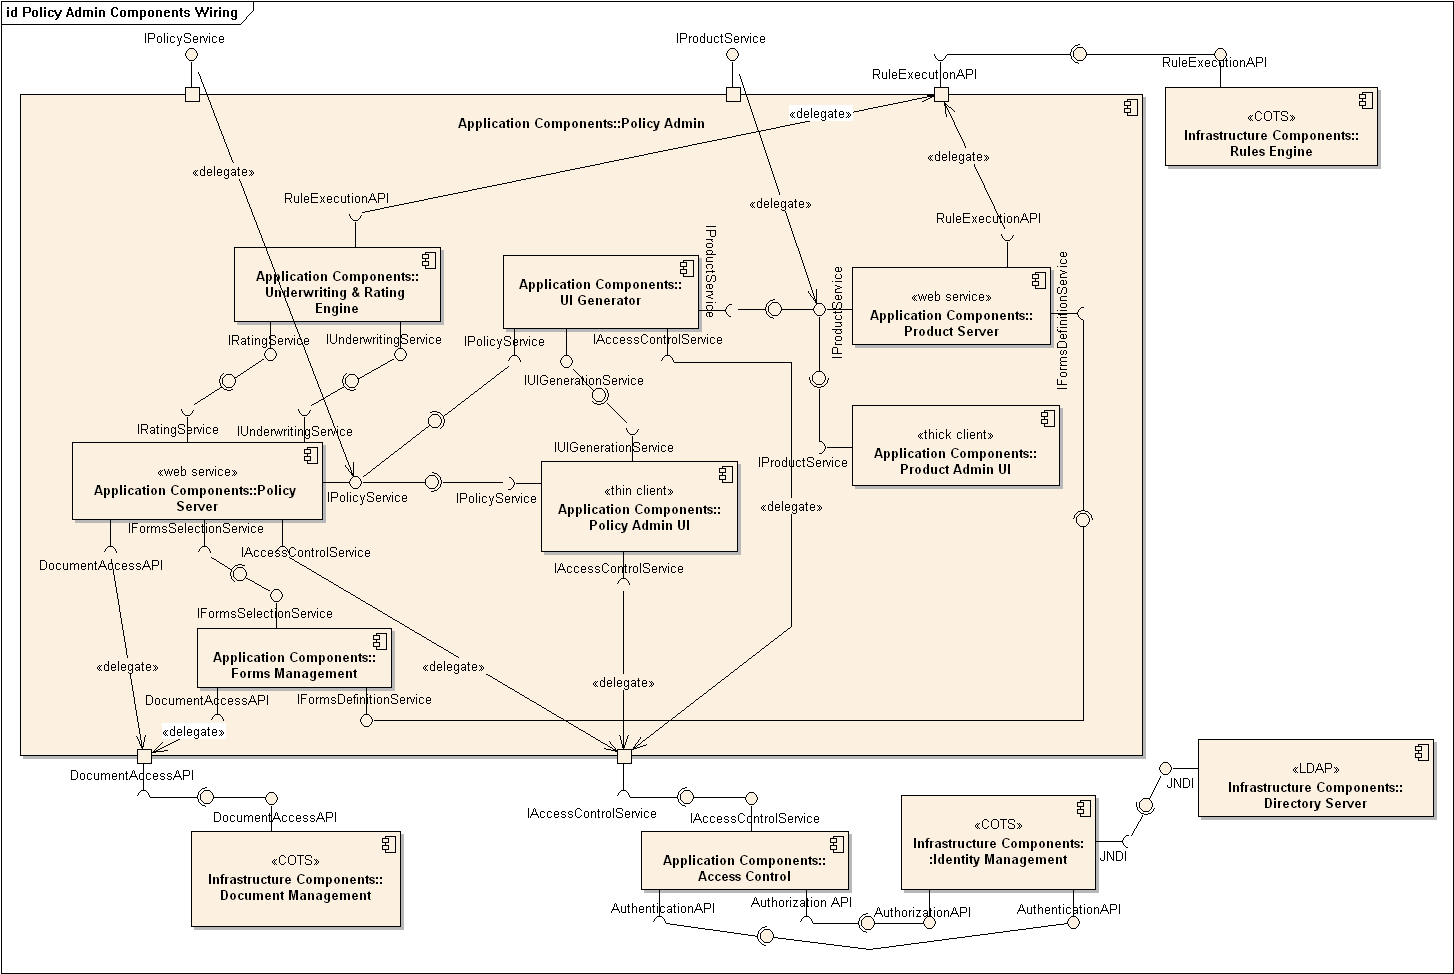
\includegraphics[width=\textwidth,height=\textheight,keepaspectratio]{Policy_Admin_Component_Diagram.png}
    \caption{Description of a software component and its inner relations in the Universal Modelling Language, \citep{wikipedia_unified_2023}}
    \label{graphic:uml}
\end{figure}

It is clear the modernists thought of function as engineering function, and aligned it with engineering aesthetics\footnote{\emph{Esthétique de l'ingénieur} is the title of one of the chapters of Le Corbusier's manifesto, \emph{Vers une Architecture} \citep{lecorbusier_vers_1923}}. Nonetheless, such a conception of function is definitely machinic, thinking of airflow, heat exchange or drainage, expressing a particular feeling of progress and achievement through industrial manufacturing techniques allowing for new material capabilities against contextual understandings.

Jacques Rancière, in his study of the Werkbund and the Bauhaus-inspired architecture, offers an alternative approach, away from the strcit functionality laid out by Sullivan and Le Corbusier before him. The simplification of forms and processes, he writes of the AEG Turbinenhalle in Berlin, which is normally associated with the reign of the machine, finds itself, on the contrary, related to art, the only thing able to spiritualize industrial work and common life \citep{ranciere_aisthesis_2013}.

Rancière offers us an additional perspective, departing form the strict function of an object or of a building, to its \emph{use}. Such a shift moves from a structure-centric perspective (such as Le Corbusier's ideal dimensions), to a human-centric perspective (such as Lacaton \& Vassal's practical extension of space and light). Peter Downton reiterates this point, when he states that "\emph{buildings and design are often judged from artistic perspectives that bear no relation to how the building’s occupants perceive or occupy the building.}" \citep{downton_knowledge_1998}. Indeed, architecture as an artform provides an immersive and systemic physical environment, thus shapes human psychology and agency within it, and forces the dweller to acknowledge and engage with their environment. This suggests that, from a formal, top-down approach which considers architecture as possessing a formal language to be realized exactly, there exists a complementary, bottom-up approach, centered around human construction and function.

% robert venturi for the learning from las vegas, but also contradiction and complexity

\subsection{Patterns and structures}
\label{subsec:patterns-structures}

A counterpoint to this modernist approach of master planning is that of Christopher Alexander. Along with other city planners in the United States, such as William H. Whythe or Jane Jacobs, Alexander belongs to an empirical tradition of determining what makes a space \emph{good} or not, by examining its uses and the feelings it elicits in the people who tread its grounds. He elaborates an approach to architecture which does not exclusively rely on abstract design and technological efficiency, but rather takes into account the multiple layers and factors that go into making

\begin{quote}
    [...] beautiful places, places where you feel yourself, places where you feel alive \citep{alexander_timeless_1979} [...]
\end{quote}

In \emph{The Timeless Way of Building}, he focuses on how beauty is involved in moving from disorganized to organized complexity, an design process which is not, in itself, the essence of beauty, but rather the condition for such beauty to arise. Alexander's conception of beauty, while very present throughout his work, is however not immediately concerned with the specifics of aesthetics, but rather with the existence of such objects. This existence, in turn, does require to be experienced sensually, including visually.

In this process of achieving organized complexity, he highlights the paradoxical interplay between symmetry and asymmetry, and pinpoints beauty as the "deep interlock and ambiguity" of the two, a beauty he also finds the the relationship between static structures of the built environment, and the flow of living individuals in their midst. In his perspective, then, architecture should take into account the role of tension between opposite elements, rather than the combination of rational and abstract design elements. Such an approach echoes other considerations of tension as a source for stimulating human engagement,such as Ricoeur's analysis of the metaphor (see \ref{subsec:literary-metaphors}), and the resolution of the riddles presented in works of obfuscated source code (see \ref{subsec:hackers}).

He therefore considers aesthetic property as a consequence of qualities such as appropriateness, rightness to fit, not-simplicit and wholeness. All of these have in common the subsequent need for a purpose, a purpose which he calls the \emph{Quality Without a Name} \citep{alexander_timeless_1979}. This quality, he says, is semantically elusive, but nonetheless exists; it is, ultimately, the quality which sustains life, a conclusion which he reached after extensive empirical research: no one can name it precisely, but everyone knows what it refers to. It is the quality which makes one feel at home, which makes one feel like things make sense in a deep, unexplicable way. This reluctance to being linguistically explicited is echoed in the work of the craftsman, where a practicioner often finds herself showing rather than telling \citep{pye_nature_2008}, another domain with which software developers identify, explicited in \ref{subsubsec:crafting-software}.

Among the adjectives used to circle around this quality are whole, comfortable, free, exact, egoless, eternal \citep{alexander_timeless_1979}. Some of these qualities can also be found in software development, particularly wholeness and comfort. A whole program is a program which is not missing any features, whose encounter (or lack thereof) might cause a crash. Conversely, it is also a program which does not have extraneous—useless—features. A comfortable program text being is a program which might be modified without fear of some unintended side-effects, without inivisible dependencies which might then compromise the whole. There is enough separation of concerns to ensure a somewhat safe working area, in which one can engage in epistemic probing assuming that things will not be breaking in unexpected ways; being whole, it also provides a higher sense of meaning by realizing how one's work relates to the rest of the construction. The implication here is that comfort derives from a certain kind of knowledge, a knowledge of how things (spatial arrangements, technical specifications, human functions) are arranged, how they relate to each other, how they can be used and modified.

To complement this theoretical pendant, Alexander conducted empirical research to find examples of such qualities, in a study led at the University of Berkley which resulted in his most popular book, \emph{A Pattern Language} \citep{alexander_pattern_1977}. In it, he and his team lists 253 patterns which are presented as to form a kind of language, akin to a Chomskian generative grammar, re-usable and extendable in a very concrete way, but without a normative, quasi-biological component. It turns it out that such a documentation, of re-usable configuration and solutions for contextual problem-solving, had a significant echo with computer scientists.

A whole field of research developed around the idea expressed in \emph{A Pattern Language}, at the crossover between computer science and architecture\footnote{See, for instance, the \emph{Beautiful Software Initiative} as an organized effort to develop Alexander's theses on growth, order, artefact and computation \citep{bryant_beautiful_2022}} of distinct, self-contained but nevertheless composable components. In Alexandrian terms, they are a triad, which expresses a relation between a certain context, a problem, and a solution. Similarly to architectural patterns, these emerged in a bottom-up fashion: individual software developers found that particular ways of writing and organizing code were in fact extensible and reusable solutions to common problems which could be formalized and shared with others. Patterns enable a cognitive engagement based on a feeling of familiarity, and of recognizing affordances. This form of engagement relies on the taking of epistemic actions in order to understand a particular system, as highlighted in \ref{subsec:psychology-programming}.

Extending from the similarities of structure and function between software and architecture mentioned above, it is the lack of learning from practical successes and failures in the field which prompted interest in Alexander's work, along with the development of Object-Oriented Programming, first through the Smalltalk language\footnote{For an extensive history of the design and development of the Smalltalk hardware and software, see \citep{kay_early_1993}}, then with C++, until today, as most of the programming languages in 2023 include some sort of object-orientation and encapsulation. What Object-orientation does, is that it provides a semantic structure to the program, reflected in the syntactic structure: objects are conceptual entities, with states and actions\footnote{In OOP, the states and actions of an object are respectively called member fields and methods}. This enables such objects to be re-used within a program text, and even across program texts.

The similarities between a pattern and an object, insofar as they are self-contained solutions to contextual situations that emerged through practice, and resulting from empirical deductions, caught on with software developers as a technical solution with a social inflection, rather than a computational focus. Writing in \emph{Patterns of Software}, with a foreword by Alexander, Richard P. Gabriel addresses this shift from the machine to the human:

\begin{quote}
    The promise of object-oriented programming—and of programming languages themselves—has yet to be fulfilled. That promise is to make plain to computers and to other programmers the communication of the computational intentions of a programmer or a team of programmers, throughout the long and change-plagued life of the program. The failure of programming languages to do this is the result of a variety of failures of some of us as researchers and the rest of us as practitioners to take seriously the needs of people in programming rather than the needs of the computer and the compiler writer. \citep{gabriel_patterns_1998}
\end{quote}

The real issue raised here in programming seems to be, again, not to speak to the machine, but to speak to other humans. This complexity of communication, had always asked to be solved, perhaps at this point in the form of object-orientation. While understanding software is hard, creating, identifying, and formalizing patterns into re-usable solutions turns out to be at least as hard \citep{taylor_patterns_2001}. Part of this comes from a lack of visibility of code bases (most of them being closed source), but also from the series of various economic and time-sensitive constraints to which developers are subject to (and echoes those in the field of architecture), and which result in moving from making something great to making something good enough to ship. The promise of software patterns seemed to offer a way out by—laboriously—codifying know-how. Interestingly, while the increase in software quality has been found to result from the application of engineering practices \citep{hoare_how_1996}, the discovery and formalization of the software patterns takes place through the format of writers' workshops\footnote{As taken from the website of the 2022 Pattern Languages of Programming conference: "At PLoP, we focus on improving the written expression of patterns through writers' workshops. You will have opportunities to refine and extend your patterns with the assistance of knowledgeable and sympathetic patterns enthusiasts and to work with others to develop pattern languages" \citep{guerra_plop_2022}.}.

Throughout his work, Gabriel draws from the work of an architect to weave parallels between his experience as a software developer and as a poetry writer, drawing concepts from the latter field into the former, and inspecting it through the lens of a pattern languages of built concrete or abstract structures. We develop further two concepts in particular, and show how \emph{habitability} and \emph{compression} enable an understanding of such structures.

\subsubsection{Compression and habitability in functional structures}
\label{subsubsec:compression-habitability}

Source code is thus also an inherently spatial medium, with entrypoints, extracted packages, parallel threads of executions, relative folders and directories and endless jump between files. Reading a program text therefore matches more closely an excursion into a foreign territory whose map might be misleading, than reading a book from start to finish. For instance, \ref{graphic:code-city} builds on a longer history of using the city as a metaphor for large code bases, and visualizes classes, packages and version in three dimensions.

\begin{figure}
    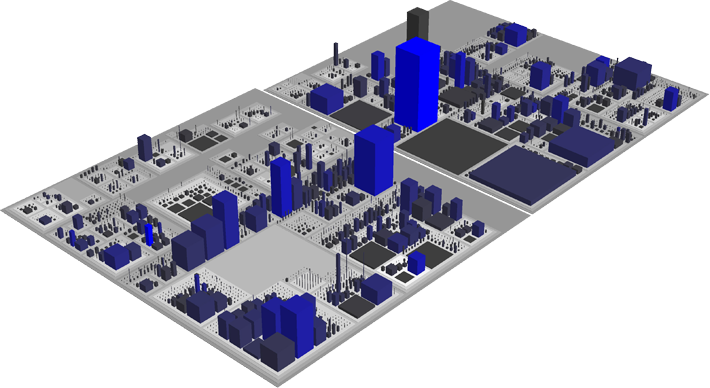
\includegraphics[width=\textwidth,height=\textheight,keepaspectratio]{codecity_screenshot.png}
    \caption{CodeCity is an integrated environment for software analysis, in which software systems are visualized as interactive, navigable 3D cities. The classes are represented as buildings in the city, while the packages are depicted as the districts in which the buildings reside. \citep{wettel_codecity_2008}}
    \label{graphic:code-city}
\end{figure}

Given this somewhat literal mapping of source code structure onto urban structure, and given the abstract structure of object-oriented code, a reader of source code will need to find their bearings and orient themselves\footnote{"Exploring a source code repository always starts with finding out what the OS will select as  the entry point. 99\% of the time it means finding the `int main(int,char**)` function" says Fabien Sanglard on the topic of reverse-engineering code-bases \citep{sanglard_game_2018}}.

One of the overlaps between architecture and software is their relation to function. Particularly in software, this relation is accompanied by the assumption that others will want to modify and extend source code. Other pieces of code might just be satisfying in being read or deciphered (as we've seen in source code poetry in \ref{subsubsec:code-poetry} or with hackers in \ref{subsec:hackers}) but this assumption of interaction with the code brings in another concept, that of \emph{habitability}. In Gabriel's terms, it is

\begin{quote}
    the characteristic of source code that enables programmers, coders, bug-fixers, and people coming to the code later in its life to understand its construction and intentions and to change it comfortably and confidently. \citep{gabriel_patterns_1998}
\end{quote}

In a sense, then, beautiful code is also code that is clear enough to inform action and, well-organized enough to warrant actually taking that action. For instance, writing in the ACM Queue, an anonymous programmer discusses the beauty in a code where the separation between which sections of the source are hardware-dependent and which are not, as seen in \ref{code:hardware-separation}. In that example, it is clear to the programmer what the problem-domain is: counter incrementation, high-performance computation, or a specific Intel chip.

\begin{listing}
    \inputminted{rust}{./corpus/hardware_separation.h}
    \caption{In the C family of languages, header files represent the overall structure of the program. This program text is defining the overall structure and the extent to which it interacts with specific hardware.}
    \label{code:hardware-separation}
\end{listing}

This distinction relates to Alexander's property of comfort, by affording involvement instead of estrangement. A specific instance of habitability, in software patterns, might be difficult to pinpoint, but can pop up in some cases: a beautiful commit is a commit which adds a significant feature, and yet only change the lines of the code that are within well-defined boundaries (e.g. a single function), leaving the rest of the codebase untouched, and yet affecting it in a fundamental way.

Still, such a feature of habitability, of supporting life, doesn't specify at all what it could, or should, look like. Rather, we get from Alexander a negative definition:

\begin{quote}
    The details of a building cannot be made alive when they are made from modular parts... And for the same reason, the details of a building cannot be made alive when they are drawn at a drawing board. \citep{alexander_timeless_1979}
\end{quote}

If modularity itself is at odds with making good (software) constructions, then its implementation under the terms of an object-oriented programming paradigm becomes complicated. Indeed, the technical formalization of the field came with the release of the \emph{Design Patterns: Elements of Reusable Object-Oriented Software} book, which lists 23 design patterns implementable in software \citep{gamma_design_1994}. Its influence (in terms of copies sold, and in terms of papers, conferences and working groups created in its wake) is undeniable, with Alexander himself giving a keynote address at the ACM two years after the release. It has, however, been met with some criticism.

Some of this criticism is that patterns are "external", they look like they come from somewhere else, and are not adapted to the code. In this sense, they join Alexander in being wary of constructions which do not integrate fully within their environments, which do not, in an organic sense, allow for a piecemeal growth\footnote{Addressing this concern, the failure of strict top-down hierarchies in software development resulted in the agile methodology for business teams}. If patterns express relations between contexts, problems and solutions, then it seems that one of the main complaints of developers looking at their code and seeing chunks of foreign code dumped in the middle to fix some generic problem\footnote{The example of the best pattern to retro-fit an air conditionner on a building would be a non-problem if the air-conditionning had been designed in from the get-go \citep{coplien_patterns_2009}.}, is the lack of understanding of context offered by those proposed solutions. In this, blindly applying patterns from a textbook might be a solution, but it's not an elegant one. This criticism also finds its echoes in the Scruton's analysis of architectural styles; rules and conventions, while present in architecture, are often adopted only to be departed from—re-interpreted and adapted to the context of the building \citep{scruton_aesthetics_2013}.

While patterns might operate at a more structural level, hinting at different parts of code, and its overall organization, one can also turn to a more micro-level. What can a detail do in our understanding of structures? Sometimes decried, sometimes praised in architecture, the detail fulfills mutliple roles: compressing meaning and testifying for materiality.

Both Scruton and Rancière mention the detail as an essential architectural element. Without contributing to the structural soundness of the construction, it nonetheless contributes to its expressiveness. A blend of the cognitive and sensual is also characteristic of Scruton's "imaginative perception", understood as the perception of the details of built structures in various ways, depending on the interpretative choices in parsing ambiguous or multiform aspects of the built environment. One of these aspects, the detail, contributes to the stylistic convention of the creation:

\begin{quote}
    Convention, by limiting choice, makes it possible to 'read' the meaning in the choices that are made \dots for style is used to 'root' the meanings which are suggested to the aesthetic understanding, to attach them to the appearance from which they are derived. \citep{scruton_aesthetics_2013}
\end{quote}

With many external constraints, due to both context and function, the architect or builder does not have much room for personal expression, and it is through details that their intent and their style are being shown. The significance of a detail can be in explaining which conventions the structure adopts, as well as communicating the intent of the creator. A significant detail manages to compress meaning into a restricted physical surface.

Compression is a concept introduced by Gabriel in response to pattern design. In narrative and poetic text, it is the process through which a word is given additional meaning by the rest of the sentence. In a sentence such as "\emph{Last night I dreamt I went to Manderley again.}" \citep{dumaurier_rebecca_1938}, the reader is unlikely to be familiar with the exact meaning of \emph{Manderley}, since this is the first sentence of the novel. However, we can infer some of the properties of Manderley from the rest of the sentence: it is most likely a place, and it most likely had something to do with the narrator's past, since it is being returned to. A similar phenomenon happens in source code, in which the meaning of a particular expression or statement can be derived from itself, or from a larger context. In object-oriented programming, the process of inheritance across classes allows for the meaning of a particular subclass to be mostly defined in terms of the fields and methods of its subclasses—its meaning is compressed by relying on a semantic environment, which might or not be immediately visible.

This, Gabriel says, induces a tension between extendability (to create a new subclass, one must only extend the parent, and only add the differentiating aspects) and context-awareness (one has to keep in mind the whole chain of properties in order to know exactly what the definition of an interface that is being extended really is). Resolving such a tension, by including enough information to hint at the context, while not over-reaching into verbosity, is a thin line of being self-explanatory without being verbose. For instance, Casey Muratori explores the process of compression in refactoring a program text, first by distinguish semantic compression from syntactic compression\footnote{"\emph{Like, literally, pretend you were a really great version of PKZip, running continuously on your code, looking for ways to make it (semantically) smaller. And just to be clear, I mean semantically smaller, as in less duplicated or similar code, not physically smaller, as in less text, although the two often go hand-in-hand.}" \citep{muratori_semantic_2014}}, and then honing in on what makes a compression successful\footnote{"\emph{Ah! It's like a breath of fresh air compared to the original, isn't it? Look at how nice that looks! It's getting close to the minimum amount of information necessary to actually define the unique UI of the movement panel, which is how we know we're doing a good job of compressing.} \citep{muratori_semantic_2014}}. Transitioning from uncompressed code (\ref{code:uncompressed}) to compressed code (\ref{code:compressed}) allows the programmer to understand broad patterns about the overall architecture of the program text—here, how to display a clickable panel on a UI widget.

\begin{listing}
    \inputminted[]{c}{./corpus/uncompressed.c}
    \caption{genalloc.c, Basic general purpose allocator for managing special purpose memory from the Linux Kernel, displaying examples of source-code spatiality \citep{muratori_semantic_2014}}
    \label{code:uncompressed}
\end{listing}

\begin{listing}
    \inputminted[]{c}{./corpus/compressed.c}
    \caption{genalloc.c, Basic general purpose allocator for managing special purpose memory from the Linux Kernel, displaying examples of source-code spatiality \citep{muratori_semantic_2014}}
    \label{code:compressed}
\end{listing}

Such a pattern does however contrast with the nature of object-oriented programming, in which inheritance (and subsequent local abstraction of subclasses) is considered best practice. Gabriel calls this idea \emph{locality}: it is

\begin{quote}
    that characteristic of source code that enables a programmer to understand that source by looking at only a small portion of it. \citep{gabriel_patterns_1998}
\end{quote}

Finally compression isn't so much a problem in poetry since, ultimately, the definitions of each words aren't quite limited to the poet's own mind but, as we've seen, also existing in the broad conceptual structures which readers hold. However, since all aspects of a program is always, and by definition, explicitly defined, programmers thus have the ultimate say on the definition of most of the data and functions described in code. Programmers create their own semantic contexts while, at the same time, having to take into account the context of the machine and the context of the problem.

In his 1951 lecture, "Building, Dwelling, Thinking", Martin Heidegger offers a perspective on these two forms of architecture: top-down and bottom-up, respectively equating them to building as erecting, and building as cultivating. To dwell is an engagement of thought and of action, one which leads to the construction of buildings in particular locations\footnote{Speaking of a farmhouse in the Schwarzwald, he describes the chain of creation as such: \emph{" A craft which, itself sprung from dwelling, still uses its tools and frames as things, built the farmhouse.}} \citep{heidegger_building_1975}. This active existence in time and space, allowing for deliberate thought and action and resulting in a better structure also equates to Gabriel's concept of habitability:

\begin{quote}
    Habitability is the characteristic of source code that enables programmers coming to the code later in its life to understand its construction and intentions and to change it comfortably and confidently \dots Software needs to be habitable because it always has to change \dots What is important is that it be easy for programmers to come up to speed with the code, to be able to navigate through it effectively, to be able to understand what changes to make, and to be able to make them safely and correctly. \citep{gabriel_patterns_1998}
\end{quote}

As Heidegger returns to the etymological root of dwelling (\emph{bauern}) in order to connect it to the possible experience of the world humans can have through language, he grounds our experience in context. His though, between earth, man, techne and construction, hints at the essence that human construction—craft—as a consequence of thought and as a precedence to construction. Taking into accoun context and materiality, a final connection between software and architecture is actually with the field that predated, and complemented, architecture: craftsmanship.

\subsection{Material knowledge}
\label{subsec:material-knoweldge}

Architecture as a field and the architect as a role have been solidified during the Renaissance \citep{pevsner_term_1942}, consecrating a separation of abstract design and concrete work. This shift obfuscates the figure of the craftsman, who is relegated to the role of executioner, until the arrival of civil engineering and blueprints overwhelmingly formalized the discipline. While computer science, through its abstract designs, echoes the modernist architect with its pure plans, the programmer, identifying itself with the craftsman, offers different avenues for knowing artefacts.

The architect emerged from centuries of hands-on work, while the computer scientist (formerly known as mathematician) was first to a whole field of practicioners as programmers, followed by a need to regulate and structure those practices. Different sequences of events, perhaps, but nonetheless mirroring each other. On one side, construction work without an explicit architect, under the supervision of bishops and clerks, did indeed result in significant achievement, such as Notre Dame de Paris or the Sienna Cathedral. On the other side, letting go of structured and restricted modes of working characterizing computer programming up to the 1980s resulted in a comparison described in the aptly-named \emph{The Cathedral and the Bazaar}. This essay described the Linux project, the open-source philosophy it propelled into the limelight, and how the quantity of self-motivated workers without rigid working structures (which is not to say without clear designs) can result in better work than if made by a few, select, highly-skilled individuals \citep{raymond_cathedral_2001,henningsen_joys_2020}.

What we see, then, is a similar result: individuals can cooperate on a long-term basis out of intrinsic motivation, and without clear, individual ownership of the result; a parallel seen in the similar concepts of \emph{collective craftsmanship} in the Middle-Ages and the \emph{egoless programming} of today \citep{brooks_mythical_1975}. The further sections will investigate how such a phenomena of building complex structures through horizontal networks is possible, from both epistemological and aesthetic perspectives.

Craftsmanship in our contemporary discourse seems most tied to a retrospective approach: it is often qualified as that which was \emph{before} manufacture, and the mechanical automation of production \citep{thompson_study_1934}, preferring materials and context to technological automation. Following Sennett, we will use his definition of craftsmanship as \emph{hand-held, tool-based, intrinsically-motivated work which produces functional artefacts, and in the process of which is held the possibility for unique mistakes} \citep{sennett_craftsman_2009}.

At the heart of knowledge transmission and acquisition of the craftsman stands the \emph{practice}, and inherent in the practice is the \emph{good practice}, the one leading to a beautiful result. The existence of an aesthetic experience of code, and the adjectives used to qualify it (smelly, spaghetti, muddy), already pointed at in \ref{subsec:lexical-fields}, already points at an appreciation of code beyond its formalisms and rationalisms, and towards its materiality. We now turn to the aesthetic experience of code within the broader context of the aesthetics of craftsmanship, highlighting code's specificity as a material.

A traditional perspective is that motor skills, with dexterity, care and experience, are an essential feature of a craftsman's ability to realize something beautiful \citep{osborne_aesthetic_1977}, along with self-assigned standards of quality \citep{pye_nature_2008,sennett_craftsman_2009}. These qualitative standards which, when pushed to their extreme, result in a craftsperson's \emph{style}, gained through practice and experience, rather than by explicit measurements \citep{pye_nature_2008} \footnote{See Pye's account of craftsmanship, and his intent to make explicit the question of quality craftsmanship and \emph{"answer factually rather than with a series of emotive noises such as protagonists of craftsmanship have too often made instead of answering it."} \citep{pye_nature_2008}}. Two things are concerned here, supporting the final result: tools and materials \citep{pye_nature_2008}. According to Pye, a craftsperson should have a deep, implicit knowledge of both, what they use to manipulate (chisels, hammers, ovens, etc.) as well as what they manipulate (stone, wood, steel, etc).

The knowledge that the craftsman derives, while being tacit (see \ref{subsec:knowing-what-how}), is directed at its tools, its materials, and the function ascribed to the artefact being constructed, and such knowledge is derived from a direct engagement with the first two, and a constant relation to the third. Finally, any aesthetic decoration is here to attest to the care and engagement of the individual in what is being constructed—its dwelling, in Heideggerian terms.

This relationship to tools and materials is expected to have a relationship to \emph{the hand}, and at first seems to exclude the keyboard-based practice of programming. But even within a world in which automated machines have replaced hand-held tools, Osborne writes:

\begin{quote}
    In modern machine production judgement, experience, ingenuity, dexterity, artistry, skill are all concentrated in the programming before actual production starts. \citep{osborne_aesthetic_1977}
\end{quote}

He opens here up a solution to the paradox of the hand-made and the computer-automated, as programming emerges from the latter as a new skill. This very rise of automation has been criticized for the rise of a Osborne's "soulless society" \citep{osborne_aesthetic_1977}, and has triggered debates about authorship, creativity and humanity at the cross-roads between artificial intelligence and artistic practice \citep{mazzone_art_2019}. One avenue out of this debate is human-machine cooperation, first envisioned by Licklider and proposed throughout the development of Human-Computer Interaction \citep{licklider_mancomputer_1960,grudin_tool_2016}. If machines, more and more driven by computing systems, have replaced traditional craftsmanship's skills and dexterity, this replacement can nonetheless suggest programming as a distinctly 21st-century craftsmanship, as well as other forms of cratsmanship-based work in an information economy.

Beautiful code, code well-written, is indeed an integral part of software craftsmanship \citep{oram_beautiful_2007}. More than just function for itself, code among programmers is held to certain standards which turn out to hold another relationship with traditional craftsmanship—specifically, form following function.

A craftsman's material consciousness is recognized by the anthropomorphic qualities ascribed by the craftsman to the material \citep{sennett_craftsman_2009}, the personalities and qualities that are being ascribed to it beyond the immediate one it posseses. Clean code, elegant code, are indicators not just of the awareness of code as a raw material that should be worked on, but also of the necessities for code to exist in a social world, echoing Scruton's analysis that architectural aesthetics cannot be decoupled from a social sense\footnote{"\emph{it is the aesthetic sense which can transform the architetct's task from the blind pursuit of an uncomprehended function into a true exercise of practical common sense.}" \citep{scruton_aesthetics_2013}}. As software craftsmen assemble in loose hierarchies to construct software, the aesthetic standard is \emph{the respect of others}, as mentioned in computer science textbooks \citep{abelson_structure_1979}.

Another unique feature of software craftsmanship is its blending between tools and material: code, indeed, is both. This is, for instance, represented at its extreme by languages like LISP, in which functions and data are treated in the same way \citep{mccarthy_lisp_1965}. In that sense, code is a material which can be almost seamlessly converted from information to information-\emph{processing}, and vice-versa; code as a material is perhaps the only non-finite material that craftspeople can work with—along with words\footnote{This disregards the impact of programming languages, the hardware they run on, and the data they process on the environment; see \citep{kurp_green_2008}}.

Code, from the perspective of craft, is not just an overarching, theoretical concept which can only be reckoned with in the abstract, but also the very material foundation from which the reality of software craftsmanship evolves. An analysis of computing phenomena, from software studies to platform studies, should therefore take into account the close relationship to their material that software developers can have. As Fred Brooks put it,

\begin{quote}
    \emph{The programmer, like the poet, works only slightly removed from pure thought-stuff. He builds his castles in the air, from air, creating by exertion of the imagination. Few media of creation are so flexible, so easy to polish and rework, so readily capable of realizing grand conceptual structures. \citep{brooks_mythical_1975}}
\end{quote}

So while there are arguments for developing a more rigorous, engineering conception of software development \citep{ensmenger_computer_2012}, a crafts ethos based on a materiality of code holds some implications both for programmers and for society at large: engagement with code-as-material opens up possibilities for the acknowledgement of a different moral standard. As Pye puts it,

\begin{quote}
    [\dots] the quality of the result is clear evidence of competence and assurance, and it is an ingredient of civilization to be continually faced with that evidence, even if it is taken for granted and unremarked. \citep{pye_nature_2008}
\end{quote}

Code well-done is a display of excellence, in a discipline in which excellence has not been made explicit. If most commentators on the history of craftsmanship, following Ruskin, lament the disappearance of a better, long-gone way of doing things, before computers came to automate everything, locating software as a contemporary iteration of the age-old ethos of craftsmanship nonetheless situates it in a longer tradition of intuitive, concrete creation.

The world of architecture has accrued its own set of design values over the years. One of those values is the principle of material honesty. One material should not be used as a substitute for another. Otherwise the end result is deceptive \citep{keith_resilient_2016}. One aspect that has been eluded so far is therefore that of the programming languages used by the programmer. Indeed, one doesn't write Ruby like one writes Java,  C++, or Lisp. If materiality is a core component of eliciting an aesthetic experience in an architectural context, then programming languages are the material of source code, and offer a specific context to the writing and reading of the program text.

A final criticism to software patterns is that they are language-independent. As such, they are often workarounds for features that a particular programming language doesn't allow from the get-go, or offers simpler implementations than the pattern's\footnote{For instance, Peter Norvig highlights that most patterns in the original book have much simpler implementations in Lisp than in C++ or Smalltalk \citep{norvig_design_1998}}.

To conclude this section, we've seen that architecture can offer us some heuristics when looking for aesthetic features which code can exhibit. Starting from the naïve understanding that form should follow function, we've examined how Alexander's theory of patterns, and its significant influence on the programming community\footnote{even spawning short-lived debates about his quality without a name on stackoverflow \citep{interstar_quality_2017}.}, points not just to an explicit conditioning of form to its function (in which case we would all write hand-made Assembly code), but rather to an elusive, yet present quality, which is both problem- and context-dependent. It is a quality that is aware of the context that the writer and reader bring with them, and of the context that it provides them, making it habitable. Software architecture and patterns aren't, however, explicitly praised for their beauty, perhaps because they disregard these contexts—by definition, they're high-level abstractions. Generic solutions are rarely elegant solutions. departing from our investigation of software as craftsmanship, and moving through towards a more abstract discipline, we turn to scientific aesthetics.

\section{Forms of scientific activity}
\label{sec:aesthetic-scientific}

% a bit more on engineering, hacking and the folly, should be explained in the beginning of modernism

As programmers learned their craft from practice and immediate engagement with their material, computer science was concomittantly developing from a seemingly more abstract discipline. Mathematicians such as Alan Turing, John Von Neumann and Grace Hopper can be seen, not as the foreparents of the discipline of computing, but rather as standing on the shoulders of a long tradition of mathematicians. Computation is, as as such, one of the many branches of contemporary mathematics and, as it turns out, such a tradition has also reccuringly included references to aesthetics. After the metaphors of literature and the patterned structures of architecture, we conclude our analysis of the aesthetic relation of domains contingent to source code by looking at how mathematics integrate formal presentation.

This section approaches the topic of aesthetics and mathematics in three different steps. First, we look at the objective or status of beauty in mathematics: are mathematical objects eliciting an aesthetic experience in and of themselves, or do they rely on the observer's perception? Considering the difference between abstract objects and their representation: is aesthetic representation ascribed to either, or to both? And what is the place of the observer in this judgment? Having  established a particular focus on the representations of abstract objects, we then turn to the epistemic value of aesthetics, and how positive aesthetic representations in mathematics can enable insight and understanding. Finally, we complement this relation between knowledge and presentation and depart from the ends of a proof, and an evaluative appraisal of aesthetics in mathematics, by investigating the actual process of doing mathematics, concluding with topics of pedagogy and ethics.

\subsection{Beauty in mathematics}
\label{subsec:beauty-mathematics}

The object of mathematics is to deal first and foremost with abstract entities, such as the circle, the number zero or the derivative, which can find their applications in fields such as engineering, physics or computer science. Because of this historical separation from the practical world through the use and development of symbols, one of the dominant discourses in the field tended to consider mathematical beauty as something intrisic to itself, and independent from time, culture, observer, or representation itself. Indeed, a circle remains a circle in any culture, and its aesthetic properties—uniformity, symmetry—do not, at first glance, seem to be changing across time or space.

According to the Western tradition, mathematics are perhaps the first art. Aristotle, in his \emph{Metaphysics}, wrote of beauty and mathematics as the former being most purely represented by the latter, through properties such as order, symmetry and definiteness\footnote{"\emph{the supreme forms of beauty are order, symmetry, and definiteness, which the mathematical sciences demonstrate in a special degree. And since these (e.g. order and definiteness) are obviously causes of many things, evidently these sciences must treat this sort of causative principles also (i.e. the beautiful) as in some sense a cause.}" \citep{aristotle_metaphysics_2006}}. By offering insight into the harmonious arrangement of parts, it was thought that mathematics could, through beauty, provide knowledge of the nature of things, providing an understanding of how things generally fit together. Beauty then naturally emerges from mathematics, and mathematics can, in turn, provide an example of beauty. At this intersection, it also becomes a source of intellectual pleasure, since gaining mathematical knowledge exercises the human being's best power—that of the mind.

Arguing for this position of objective quality being revealed through beautiful manifestation, Godfrey H. Hardy writes, in his \emph{Mathematician's Apology}, that beauty is constitutive of the objects that compose the field; their abstract quality is what removes them from the contextuality of human judgment.

\begin{quote}
    A mathematician, like a painter or a poet, is a maker of patterns. If his patterns are more permanent than theirs, it is because they are made with \emph{ideas}. A painter makes patterns with shapes and colours, a poet with words.
    \dots
    The mathematician's patterns, like the painter's or the poet's must be \emph{beautiful}; the ideas like the colours or the words, must fit together in a harmonious way. Beauty is the first test: there is no permanent place for ugly mathematics. \citep{hardy_mathematician_2012}
\end{quote}

It is the arrangement of ideas that possess aesthetic value, and not the arrangement of the representation of ideas. In this, he follows the position of other influential mathematicians, such as Poincaré \citep{poincare_science_1908}, or Dirac \citep{kragh_paul_2002}, who rely on beauty as a property of the mathematical object in itself. For instance, Dirac states that a physical law must necessarily stem from a beautiful mathematical theory, thus asserting that the epistemic content of the theory and its aesthetic presentation are inseparable; a good mathematical theory is therefore intrinsically beautiful. Summing up these positions, Carlo Cellucci establishes proportion, order, symmetry, definiteness, harmony, unexpectedness, inevitablity, economy, simplicity, specificity,  and integrations as the different properties inherent to mathematical objects, as mentioned from an essentialist perspective \citep{cellucci_mathematical_2015}. Ironically, this rather seems to hint at the multiplicity of appreciations of beauty within mathematics, with mathematicians concurring on the existence of beauty, but not agreeing on what kind of beauty pertains to mathematics. Nonetheless, they do agree that beauty is connected to understanding and epistemic acquisition. John Von Neumann, writing in 1947, states that:

\begin{quote}
    One expects a mathematical theorem or a mathematical theory not only to describe and to classify in a simple and elegant way numerous and a priori disparate special cases. One also expects "'elegance" in its "architectural," structural makeup. Ease in stating the problem, great difficulty in getting hold of it and in all attempts at approaching it, then again some very surprising twist by which the approach, or some part of the approach, becomes easy, etc\dots \citep{vonneumann_mathematician_1947}
\end{quote}

The point that Von Neuman makes here is a difference between the content of the mathematical object and its structural form. Such a structural form, by organizing the connection of separate parts into a meaningful whole, makes it easy to grasp the problem. In this sense, it is both the crux of aesthetics and the crux of understanding. Similarly, Francois Le Lionnais, a founding member of the Oulipo literary movement in postwar France, wrote an essay on the aesthetic of mathematics, paying attention to both the mathematical objects in and of themselves, such as e or π, but also to mathematical methods, and how they compare to traditional artistic domains such as classicism or romanticism. Without getting into the intricacies of this argumentation, we can nonetheless note that his descriptions of mathematical beauty find echoes in source code beauty. For instance, his appraisal of the proof by recurrence\footnote{"\emph{It seems to us that a method earns the epithet of classic when it permits the attainment of powerful effects by moderate means. A proof by recurrence is one such method. What wonderful power this procedure possesses! In one leap it can move to the end of a chain of conclusions composed of an infinite number of links, with the same ease and the same infailliability as would enter into deriving the conclusion in a trite three-part syllogism."}" \citep{lelionnais_great_1971}} reflects similar lines of praise given by programmers to the elegance of recursive functions, which are sharing the same mathematical device (for instance, see \ref{code:recursion_iteration_csharp} and \ref{code:scheme_interpreter} for examples of recursion as an aesthetic property). A proof by recurrence is indeed a kind of structure, which can be adapted to demonstrate different kinds of mathematical objects.

To understand is to grasp how each elements fits with others within a greater structure (either in a poem, a symphony or a theorem), with each of these elements being rendered sensible to the observer \citep{cellucci_mathematical_2015}. The beauty of a mathematical object can then be ascribed in its display of the definite relation between its elements. For instance, the equation representing Euler's identity (see \ref{graphic:euler}) demonstrates the relation between geometry, algebra and numerical analysis through a restrained set of syntactic symbols, where e is Euler's number, the base of natural logarithms, i is the imaginary unit, which by definition satisfies i\^{2} =-1, and π is the ratio of the circumference of a circle to its diameter. Each of the symbols is necessary, definite, and establishes clear relations between each other, revealing a deep interlock of simplicity within complexity.

\begin{figure}
    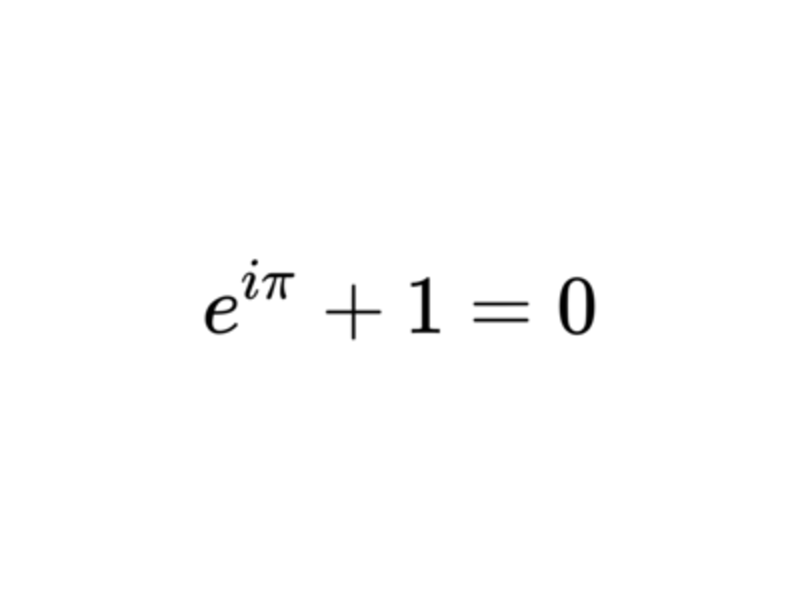
\includegraphics[width=\textwidth,height=\textheight,keepaspectratio]{euler.png}
    \caption{Euler's identity demonstrates the relation between geometry, algebra and numerical analysis through a restrained set of syntactic symbols.}
    \label{graphic:euler}
\end{figure}

This equation ranked first in a column in the \emph{Mathematician Intelligencer} about the beauty of mathematical objects; the columnist, David Wells, had asked readers to rank given theorems, on a linear scale from 0 to 10, according to how beautiful they were considered \citep{wells_are_1990}\footnote{Along with, for instance, the infinite prime theorem, and Fermat's "two squares" theorem.}. Again, while this assessment does show that there can be consensus, and thus some aspect of objectivity, in a mathematicians' judgment of beauty in a mathematical object, it also showed that mathematical beauty also depends on the observer, since mathematicians' provided varying accounts.

Rather than focusing on the beauty of the mathematical entities themselves, then, another perspective is to consider beauty to be found in the \emph{representation} of mathematical entities. This disjunctive view, that aesthetics and mathematics can be decoupled (there can be ugly proofs of insightful theorems, and elegant proofs of boring theorems), was first touched upon by Kant. As Starikova highlights, the philosopher operates a distinction between perceptual, disinterested beauty, and intellectual, vested beauty. Perceptual beauty, the one which can be found in the visual representations of mathematical entities, is the only beauty graspable, while intellectual beauty, that of the objects themselves, simply does not exist, "mathematics by itself being nothing but rules" \citep{starikova_aesthetic_2018}.

Such manifestation of perceptual beauty can be found in the phenomenon of re-proving in existing proofs, in order to make them more beautiful; Rota, for instance, associates the beauty of a piece of mathematics with the shortness of its proof, as well as with the knowledge of the existence of other, clumsier proofs\footnote{"\emph{"The beauty of a piece of mathematics is frequently associated with shortness of statement or of proof.}" and \emph{"A proof is viewed as beautiful only after one is made aware of previous, clumsier proofs.}" \citep{rota_phenomenology_1997}} \citep{rota_phenomenology_1997}. Thus, it is not so much the content of the proof itself, nor the abstract mathematical object being proven that is the focus of aesthetic attention, but rather the process of establishing the epistemic validity of such an object.

What is useful here is \emph{technique}, the demonstration of the knowledge from the prover to the observer, through the proof. As such, the asssessment of aesthetics in mathematics, both as a producer and as an observer, depends highly on the expertise of each individual, and on the previous knowledge that this indivual has of mathematics\footnote{"\emph{Mathematical creation is not so free, hence the contrasting analogy of the landscape gardener, who needs a good grasp of the topography before getting down to creating something beautiful which needs to be based on that topography.}" \citep{thomas_beauty_2017}} \citep{thomas_beauty_2017} (an assessment of the aesthetics of mathematics for non-expert is discussed in \ref{subsec:aesthetics-heuristics} below). It seems that the way that the mathematical object is presented does matter for the assessment.

If beauty is not intrinsic to the mathematical object, but rather connected to the presentation of the mathematician's knowledge, there remains the question of why is beauty taken into account in the doing of mathematics. Looking at the lexical fields used by mathematicians to qualify their aesthetic experience, as reported in \citep{inglis_beauty_2015} provides us with a clue: amongst the most used terms are "ingenious", "striking", "inspired", "creative", "beautiful", "profound" and "elegant". Some of these terms have a connection to the epistemic: for instance, something ingenious enables previously unseen connections between concepts, implying the resourcefulness and the cleverness of the originator of the idea. The next question is therefore that of the relationship between the aesthetic and the epistemic in mathematics; and in how this relation can manifest itself in source code.

\subsection{Epistemic value of aesthetics}
\label{subsec:epistemic-aesthetics}

Caroline Jullien offers an alternative to the perception of mathematics as an autotelic aesthetic object, by retracing the definitions of beauty given by Aristotle and establishing a cognitive connection through a cross-reading of the \emph{Metaphysics} and the \emph{Poetics}, highlighting that "the characteristics of beauty are thus useful properties that yield an optimal perception of the object they apply to. [...] Men can understand what is ordered, measured and delineated far better than what is chaotic, without clear boundaries, etc." \citep{jullien_languages_2012}. She then develops this point further, developing from Poincaré's assessment of mathematical entities which fulfill aesthetic requirements and are, at the same time, an assistance towards understanding the whole of the mathematical object presented. Aesthetics, then, might not exist exclusively as intrinsic properties of a mathematical object, but rather as an epistemic device, as aesthetic properties might thus be conceived as cognitive properties. 

Her argument focuses on considering mathematics as a language of art in the Goodmanian sense of the term, investigating how mathematical notation relates to Goodman's criteria of syntactic density, semantic repleteness, semantic density, exemplification and multiple references \citep{jullien_languages_2012}. She shows that, while mathematical notation might not seem to satisfy all criteria (for instance, syntactic density is only fulfilled if one takes into account graphical representations), a mathematical reasoning can be analyzed as a symptom of art, particularly through the ability to exemplify and refer to abstract entities.

However, to do that, she also includes different representations of mathematical systems, beyond typographical characters. Including diagrams and graphs, it becomes easier to see how a more artistic representation of mathematics is possible. The thickness of a line, the color-coding or the spatial relationship can all express a particular class of mathematical objects; for instance, the commutative property in arithmetic can be represented in geometry through the aesthetic property of symmetry. In this work, we focus on the textual representation of source code, eluding any graph or diagram (such as the one we've seen in architectural descriptions of software systems in \ref{graphic:uml}). Nonetheless, we have argued in \ref{sec:aesthetic-scientific} that source code qualifies as a language of art: while the syntactic repleteness does not match that of, say, painting, the unlimited typographical combinations, paired with the artificial design of programming languages as working medium enables the kinds of subtle distinctions necessary for symptoms of the aesthetic to be present.

Following Jullien, if a piece of mathematics is eliciting an aesthetic experience, or presenting positive aesthetic properties, it might then be a support for the understanding by the viewer of this very piece of mathematics. Such a support is itself manifested in this ability to manifest a harmonious correspondence of parts in relation to a whole. A beautiful presentation is a cognitively encouraging presentation. The subsequent question then regards the nature of that understanding: if it does not happen as an instant stroke of enlightenment, how does it take place as a gradual process of deciphering \citep{rota_phenomenology_1997}?

Addressing this question, Carlo Celluci suggests that a hint lies in the concept of fitness, meaning the appropriateness of a symbol in its denotation of a concept, and the appropriateness of concepts in their demonstration of a theorem. Only through this dual level can fitness enable understanding rather than explanation \citep{cellucci_mathematical_2015}. This gradual conception of understanding fits the context of proofs and demonstration; when confronted with source code—that is, with the result of a thought process of one or more programmers—the processual conception of understanding seems to find its limits. For instance, the linked list shown in \ref{code:linked_list} establishes a very concise representation of a list, and holds within it thoughtful implications in terms of organizing and accessing sequential data. However, it is limited in communicating why this is a canonical example of such a computational entity, or how did one reach this conclusion among other possible entites.

\begin{listing}
    \inputminted{c}{./corpus/linked_list.h}
    \caption{A textbook example of a fundamental construct in computer science, the linked list. This header file shows all the parts which compose the concept \citep{kirchner_content_2022}.}
    \label{code:linked_list}
\end{listing}

Looking at \ref{code:linked_list}, one can view the different relationships between parts and wholes: the list item composing the list itself, the head pointer being a specific instance of the next pointer, and the different methods to access or modify the list itself. Seeing all of these together suggest an understanding of the whole through the parts which is nowhere explicitly described but everywhere suggested.

Similarly, the example shown in \ref{code:regex} highlights some of the similarities between source code aesthetics and the aesthetics of mathematics. Featured in \emph{Beautiful Code} edited volume, this listing shows the essential components of a regular expression matcher. Regular expressions are a form of linguistic pattern that serve as an input to a regular expression matcher in order to find particular patterns of text in an input string. In this case, the essential components of the matcher are implemented, in a clear and concise way. It highlights the process of looping over an input string, the fundamentals of handling different patterns, and within those the fundamentals of handling different characters in relation to the current pattern. Each part is clearly delineated (and thus fit for its separate purposes) and contributes to an understanding of the whole, by limiting itself to displaying its essence.

\begin{listing}
    \inputminted{c}{./corpus/regex.c}
    \caption{A regular expression matcher by Rob Pike, praised for its elegance and conciseness, but not for its utility \citep{oram_beautiful_2007}}
    \label{code:regex}
\end{listing}

Mathematics, like source code, therefore pay close attention to how formal presentation facilitates the cognitive grasping of abstract concepts. Reducing and organizing literal tokens into conceptually coherent units, and meaningful relations to other units—for instance, having the code in \ref{code:regex} reversed, with the \lstinline{match()} function at the bottom of the document would represent a different level of importance of that entrypoint function, which would complicate the understanding of how the source code functions.

Another overlap between aesthetics in source code and aesthetics in mathematics is the attention that needs to be paid to skill and context. In order to appreciate the regular expression matcher aesthetically, one must know that this is an essential representation of a matcher, and not a functionally complete representation of matcher (\ref{code:regex} misses some edge cases to make it usuable). Someone operating in a functional context might find this representation lacking and useless, while concise. Similarly, the linked list example (see \ref{code:linked_list}) might be considered aesthetically pleasing only at a particular level of skill. Indeed, as we see in \ref{code:linked_list_remove}, the distinction is clearly made between a beginner level (labelled "CS101" for the course number of introduction to computer science) and a non-beginner (meaning, elegant) level.

\begin{listing}
    \inputminted{c}{./corpus/linked_list.c}
    \caption{A comparison of how to remove an element from a list, with elegance depending on the skill level of the author \citep{kirchner_content_2022a}.}
    \label{code:linked_list_remove}
\end{listing}

At this point, we should note that some argue for aesthetics as a subset cognitive properties. For instance, Starikova that "\emph{[A]lthough visual representations are involved and understanding does rely on them, it is clearly non-perceptual beauty that initiates aesthetic judgment}" \citep{starikova_aesthetic_2018}, pointing back to the distinction above as to whether beauty is perceived as intrinsic to the mathematical object, or intrinsic to its representation. Here, we argue that both approaches in source code—intellectual engagement eliciting aesthetic pleasure, and aesthetic pleasure eliciting intellectual engagement—are not mutually exclusive. Specifically, these depend on the nature of background knowledge that the reader holds when engaging with a program text. On one side, the pre-existence of knowledge allows one to focus on the quality and details of the presentation, such as when mathematicians decide to find more beautiful proofs to an existing theorem. In this case, the knowledge of the theorem, and how its intellectually-perceived simplicity can be translated into a sensually-perceived simplicity and an aesthetic judgment on the form. On the other side, the lack of pre-existing knowledge involves the deciphering of symbols and thus immediate attention to form. Here, the aesthetic judgment precedes the intellectual judgment, all the while not guaranteeing a positive intellectual judgment (e.g. the abstract object, whether program function or mathematical theorem, is presented in an aestheticlly-pleasing manner, but remains shallow, boring, non-sensical or wrong).

We consider here that both intellectual pleasure and aesthetic pleasure happen in a dialogic fashion, considering the symbols and the meanings reciprocally, until intellectual and aesthetic judgments have been given. This is in line with Rota's critique of the term "enlightenment" or "insight" in his phenomenological account of beauty in mathematics. The process of discovery and understanding is a much longer one than a simple stroke of genius experienced by the receiver \citep{rota_phenomenology_1997}.

An aesthetic experience in mathematics involves uncovering the connections between aesthetic and epistemic value being represented through a mathematical sumbol system. However, such a conception seems to take place as a gradual process of discovery, both from the writer and from the reader. Seen in the light of skill-based aesthetic judgment, this chronological unfolding points towards a final aspect of aesthetics in mathematics specifically, and in the sciences in general: aesthetics as heuristics for knowledge acquisition.

\subsection{Aesthetics as heuristics}
\label{subsec:aesthetics-heuristics}

Harold Osborne (same guy who was writing about craftsmanship): "the reliance on the heuristic value of mathematical beauty in scientific theory has become something of a commonplace"
% https://academic.oup.com/bjaesthetics/article/24/4/291/28880
% https://academic.oup.com/bjaesthetics/article/4/2/160/98684

So far, we had been looking at how aesthetics are evaluated in a finished state—that is, once the form of the object (whether a proof or a program text) has stabilized. In doing so, we have left aside a significant aspect of the matter. Aesthetics in mathematics do not need to be seen exclusively as an end, but also as a mean, as a part of the cognitive process engaged to achieve a result.

% 1k on nathalie sinclair, her distinction between different kinds of roles that aesthetics have
% 3k on the generative and motivational value of aesthetics, of heuristics (remind the structural engineer that used to say to choose designs that are good because they look good)
% 1k on dewey and his theory of inquiry: PERSONAL

Nathalie Sinclair: evaluative role, generative role, motivational role. the generative role is the one that is guiding and activates the process of inquiry: generates new ideas and insights (both positively and negatively, i.e. when something looks bad and needs to be fixed because we know there's a way that it can look good)

\begin{quote}
    The aesthetic capacity of the student relates to her sensibility in combining information and imagination when making purposeful decisions, regarding meaning and pleasure. This is a use of the term aesthetic drawn from interpretations such as dewey \citep{sinclair_roles_2004}
\end{quote}

She connects it with Dewey's theory of inquiry (1938) and with Polanyi's personal knowledge theory, getting further into psychological perception and/or role of aesthetics.

% 1k on papert, and the functional role of aesthetics as a guide to figure out how to do mathematics
% particularly, we mention his reliance on Piaget, but also this idea of comparative aesthetics: gestalt vs sequential
% and we solve this lack of sequentiality with refactoring
% and we even include some code, showing the process of refactoring

% 2k move from PERSONAL to SOCIAL: on the social role of aesthetics: style, convention, value

\begin{quote}
    Pimm's framing offers an avenue of inquiry that shifts attention from the modes of mathematical inquiry of individual mathematicians, as Sinclair's tripartite model, to the practices of the community as a whole, including how truths are named, manipulated and negotiated. \citep{sinclair_aesthetic_2011}
\end{quote}

% also include this relation to the ethical paper (beautiful code is code of someone who cared)

%2k expand with bernstein to the rest of sciences
Root Bernstein broadens this all of scientific activity, not just mathematics. Feelings and emotions are prime allies of investigation, through motivation and attraction, and thus for supporting creative scientific activity.

\begin{quote}
    I propose four major arguments. First, all scientific problem solving and problem generation involves emotional and sensual responses that are similar if not identical to those associated with the arts. Second, that the experience of knowing what one feels and feeling what one knows constitutes a specific form of understanding that I call “synosia”. Third, there is a “meta-logic” to these intuitive responses that is embedded in what we call scientific aesthetics. Fourth, that aesthetic cognition precedes and is distinct from formal logic, and that an explicit translation process is therefore required before ideas can be communicated and tested logically. In sum, aesthetic cognition combines knowledge and feeling into synosic intuition that has an analyzable “meta-logic” which is the basis for creative scientific thinking. \citep{root-bernstein_aesthetic_2002}
\end{quote}

\begin{quote}
    The realization that we recognize problems through our anti-aesthetic response to them provides an important clue as to how we go about deŽ ning the nature of the problem and recognize its solution. The nature of the disjuncture between our aesthetic expectations and what we observe or think we know reveals the detailed characteristics of the specific problem that presents itself. \citep{root-bernstein_aesthetic_2002}
\end{quote}

"It remains to reify this meta-logic as a set of rules, axioms, or practices.", which is a good segue into the final chapter

He says that the informal insights of aesthetic intuition precede formal logic. Only when we explicitly recognize that the “tools of thinking” and the “tools of communication” are distinct can we understand the intimate, yet tenuous, connection between thought and language, imagination and logic.

\spacer

In conclusion, we have seen that there is a clear connection between aesthetics and cognition, and that it exists across domains. For literature, it is about accessing three-dimensional space through two-dimensional surface and one-dimensional sentences. For architecture, it is about cognition as ability to modify and act within, as well as the ability to derive the meaning of things from their appearances. In mathematics, it is about compressing the maximum amount of insight (which is different from just knowledge) in the minimum amount of explanation/tokens. For engineering it's not quite sure yet, but it's related to architecture: how functional (in the social and technical sense) it is.
